%#######################################
% Original: Oktober.2011; Prof. Dr. Martin Grüttmüller, FIM
% Last Edit: Dezember.2021; M.Eng. Mario Hoffmann, Fakultät DIT
% Reimport: April.2022; Prof. Dr. Jean-Alexander Müller, Fakultät Informatik und Medien
%#######################################

%!TEX TS-program = lualatex
%!TEX encoding = UTF-8 Unicode
%!TEX root = Bachelorarbeit.tex
%!TEX spellcheck = de_DE
%!BIB program = biber

\documentclass[
    a4paper,
    12pt,
    numbers=noenddot,
    parskip,
    toc=flat,
    toc=listof,
    toc=bibliography,
    twoside=false,
    captions=tableheading]{scrbook}


%##########################################################
% Einbinden aller Pakete etc.
%##########################################################

%!TeX root = ./../Bachelorarbeit.tex

%##########################################################
% Dokumentenangaben
%##########################################################

% ---- Studiengang ----
\newcommand{\studiengang}{Informatik}
\newcommand{\studienganggrad}{Bachelor of Science}
\newcommand{\fakultaet}{Informatik und Medien}
\newcommand{\hochschule}{Hochschule für Technik, Wirtschaft und Kultur}

% ---- Autor + Gutachter ----
\newcommand{\autor}{Jonas Schulze}
\newcommand{\geburtsort}{Hohenmölsen}
\newcommand{\geburtstag}{23.04.2001}

\newcommand{\erstgutachter}{Prof. Dr.-Ing. Jean-Alexander Müller}
\newcommand{\instituteErstgutachter}{HTWK Leipzig}
\newcommand{\zweitgutachter}{M. Sc. Robin Escherich}
\newcommand{\instituteZweitgutachter}{SENEC GmbH}

% ---- Titel, etc ----
\newcommand{\abschlussarbeit}{Bachelorarbeit}
\newcommand{\titel}{Emulation eines 32 Bit Mikrocontrollers zur virtualisierten Ausführung einer Embedded Software Applikation}
% Falls kein Untertitel, einfach leer lassen
\newcommand{\subtitel}{}
\newcommand{\ort}{Leipzig}

% ---- Betreuender Betrieb ----
\newcommand{\betrieb}{SENEC GmbH}

%!TeX root = ./../Bachelorarbeit.tex


%##########################################################
% Pakete - Stil, Sprache und Schriftart
%##########################################################
\usepackage[UKenglish,ngerman]{babel}
\usepackage[T1]{fontenc}
\usepackage[osf,scale=1.15]{sourcesanspro}
\usepackage{csquotes}
\usepackage[headsepline]{scrlayer-scrpage}
\usepackage{fontspec}
\setcounter{tocdepth}{\subsubsectiontocdepth}
\addtokomafont{chapterentry}{\bfseries}
\usepackage[onehalfspacing]{setspace}
%## #### #### ####### ###
\usepackage[absolute, overlay]{textpos}
\usepackage{svg}

% Bib Literatur Verweise
\usepackage[
	backend=biber,
	style=numeric,
	bibencoding=utf8]{biblatex}
\addbibresource{Literatur.bib}

\AtBeginDocument{%
	\providecaptionname{ngerman}{\lstlistlistingname}{Quellcodeverzeichnis}
	\providecaptionname{ngerman}{\lstlistingname}{Quellcode}
}

%##########################################################
% Pakete - Grafisches Elemente und Farben
%##########################################################
\usepackage{graphicx}
\usepackage{xcolor}

\providecommand{\keywords}[1]{\textbf{\textit{Keywords:}} #1}

%############ HTWK Farben #################
\xdefinecolor{htwkGelb}{rgb}{0.996,0.925,0}
\xdefinecolor{htwkGrau}{rgb}{0.945,0.945,0.945}
\xdefinecolor{htwkBlau}{rgb}{0,0.273,0.597}
\xdefinecolor{htwkMagenta}{rgb}{0.894,0,0.488}
\xdefinecolor{htwkRot}{rgb}{0.894,0.1875,0.035}
\xdefinecolor{htwkGruen}{rgb}{0,0.586,0.304}
\xdefinecolor{htwkCyan}{rgb}{0,0.617,0.886}
\xdefinecolor{codegreen}{rgb}{0,0.6,0}
%######## Legen Sie die Farbe fest #####
% htwkBlau, htwkGruen, htwkRot, htwkCyan, htwkGelb, htwkMagenta, htwkGrau
\newcommand{\farbe}{htwkBlau}
\newcommand{\urlfarbe}{htwkBlau}
\newcommand{\citefarbe}{htwkBlau}
%#########################################

% Linkformatierung
\usepackage[
	    colorlinks=true,
	    urlcolor={\urlfarbe},
	    citecolor={\citefarbe},
		pdftitle={\titel},
		pdfauthor={\autor},
		breaklinks=true,
		hidelinks
]{hyperref}

%##########################################################
% Pakete - Zusätzliche
%##########################################################

\usepackage{listings}
\usepackage{scrhack}
\usepackage{microtype}
\usepackage{acro}
% Used for subfigure command
\usepackage{subcaption}

%##########################################################
% Code Snippet Definitionen
%##########################################################
\newcommand\digitstyle{\color{black}}
\makeatletter
\newcommand{\ProcessDigit}[1]
{%
  \ifnum\lst@mode=\lst@Pmode\relax%
   {\digitstyle #1}%
  \else
    #1%
  \fi
}

\lstdefinestyle{MyStyle}{
	basicstyle=\footnotesize\sffamily,
	keywordstyle=\color{blue},
	commentstyle=\color{codegreen},
	stringstyle=\color{orange!80!black},
	morecomment=[l]{//},
	morecomment=[l]{/*}{*/},
	morestring=[b]",
	morestring=[b]',
	breakatwhitespace=false,
    breaklines=true,
    keepspaces=true,
	showspaces=false,
    showstringspaces=false,
    showtabs=false,
    tabsize=2,
	numbers=left,
	numberstyle=\tiny,
	frameround=tttt,
	frame=trbl,
	columns=fullflexible,
	xleftmargin=0.03\linewidth,
	xrightmargin=0.01\linewidth,
	inputencoding=utf8,
}

\lstset{
	style=MyStyle,
	literate=%
    {0}{{{\ProcessDigit{0}}}}1
    {1}{{{\ProcessDigit{1}}}}1
    {2}{{{\ProcessDigit{2}}}}1
    {3}{{{\ProcessDigit{3}}}}1
    {4}{{{\ProcessDigit{4}}}}1
    {5}{{{\ProcessDigit{5}}}}1
    {6}{{{\ProcessDigit{6}}}}1
    {7}{{{\ProcessDigit{7}}}}1
    {8}{{{\ProcessDigit{8}}}}1
    {9}{{{\ProcessDigit{9}}}}1
}

%!TeX root = ./../Bachelorarbeit.tex

%##########################################################
% Inhalt
%##########################################################

\DeclareAcronym{htwk}{
    short = HTWK,
    long = Hochschule für Technik{,} Wirtschaft und Kultur Leipzig
}

\DeclareAcronym{fim}{
    short = FIM,
    long = Fakultät Informatik und Medien
}

\DeclareAcronym{can}{
    short = CAN,
    long = Controller Area Network
}

\DeclareAcronym{ram}{
    short = RAM,
    long = Random Access Memory
}

\DeclareAcronym{arm}{
    short = ARM,
    long = Advanced RISC Machines
}

\DeclareAcronym{cpu}{
    short = CPU,
    long = Central Processing Unit
}

\DeclareAcronym{jtag}{
    short = JTAG,
    long = Joint Test Action Group
}


%##########################################################
% Begin des Dokumentes
%##########################################################
\begin{document}

%!TeX root = ./../Bachelorarbeit.tex

\pagestyle{scrheadings}
\clearpairofpagestyles

\ofoot[\pagemark]{\pagemark}
\ohead{\headmark}
\automark{chapter}

%!TeX root = ./../Bachelorarbeit.tex

%##########################################################
% Titelseite
%##########################################################

\begin{titlepage}
	\noindent
\begin{textblock*}{4.74cm}(16.7mm,11mm)

\includegraphics[width=4.74cm]{anlagen/bilder/logos/HTWK-Fakultaetszusatz_IM_schwarz_de-eps-converted-to.pdf}
\end{textblock*}
\begin{center}

\vspace*{0.5cm}

\large
{\textsc{\Large \abschlussarbeit}}

\vspace*{0.5cm}
zur Erlangung des akademischen Grades\\[0.6cm]
\studienganggrad\\[0.6cm]
im Studiengang \studiengang\\
der Fakultät \fakultaet\\
der \hochschule\ \ort\\

{\LARGE \textbf{\titel}}\\
{\LARGE \textbf{\subtitel}}

\end{center}

%##########################################################
% Autor/in
%##########################################################

\vspace*{2cm}
vorgelegt von: \autor\\
Geburtsort: \geburtsort\\
Geburtsdatum: \geburtstag\\
Abgabe: \ort, den \today


\vspace*{1cm}
\large
\begin{tabbing}
\hspace{4cm}\=\kill
Erstgutachter:  \> \erstgutachter, \instituteErstgutachter\\ 
Zweitgutachter: \> \zweitgutachter, \instituteZweitgutachter\\
\end{tabbing} 

\begin{textblock*}{8.41cm}(18mm,268.3mm)

\includegraphics[width=8.41cm]{anlagen/bilder/logos/htwk-logo-eps-converted-to.pdf}
\end{textblock*}

\end{titlepage}


%##########################################################
% Sperrvermerk
% Ist vorher abzuklären!
%##########################################################
\pagenumbering{gobble}
%%!TeX root = ./../MusterAbschlussarbeit.tex

%##########################################################
% Inhalt
%##########################################################

\thispagestyle{empty} % no page number
\chapter*{Sperrvermerk}

\noindent
Die vorliegende Bachelorarbeit mit dem Titel \titel{} beinhaltet interne vertrauliche Informationen der Firma \betrieb{} des Autors oder patentrechtlich relevante Informationen. 

Die Weitergabe des gesperrten Inhaltes der Arbeit und eventuell beiliegender
Zeichnungen und Daten im Gesamten oder in Teilen ist grundsätzlich untersagt. Es dürfen keinerlei Kopien oder
Abschriften -- auch in digitaler Form -- gefertigt werden. 
Ausnahmen bedürfen der vorherigen schriftlichen Genehmigung der Firma \betrieb{} oder des Autors.

%Hier kommen die Unterschriften hin
\vspace{1.5cm}
\begin{tabular}{p{7cm}p{.5cm}p{7cm}}
	\dotfill & & \dotfill \\\\
	Ort, Datum, Unterschrift \erstgutachter & & Ort, Datum, Unterschrift \zweitgutachter \\
    & & \\\\
    & & \\\\
    \dotfill \\\\
    Ort, Datum, Unterschrift \autor
\end{tabular}


%##########################################################
% Eidesstaatliche Erklärung
%##########################################################
%!TeX root = ./../Bachelorarbeit.tex

%##########################################################
% Inhalt
%##########################################################

\clearpage
\thispagestyle{empty}
\chapter*{Eidesstattliche Erklärung}

Hiermit erkläre ich, dass ich die an der Hochschule für Technik, Wirtschaft und Kultur Leipzig, konkret an der \ac{fim}, eingereichte Arbeit zum Thema \titel{} selbstständig, ohne Hilfe Dritter und ohne Benutzung anderer als der angegebenen Quellen und Hilfsmittel verfasst habe. 

Alle den benutzten Quellen wörtlich oder sinngemäß entnommenen Stellen sind als solche einzeln kenntlich gemacht. Die Abbildungen in dieser Arbeit wurden von mir selbst erstellt oder mit einem entsprechenden Hinweis auf die Quelle versehen.

Diese Arbeit ist bislang keiner anderen Prüfungsbehörde vorgelegt und auch nicht veröffentlicht worden.

Ich bin mir bewusst, dass eine falsche Erklärung rechtliche Folgen haben wird.

\noindent

\vspace{3cm}
\begin{tabular}{p{7cm}p{.5cm}}
    \dotfill \\\\
    Unterschrift \autor\\
    \ort, den \today
\end{tabular}


%##########################################################
% Vorwort (optional)
%##########################################################
%!TeX root = ./../MusterAbschlussarbeit.tex

%##########################################################
% Inhalt
%##########################################################
\clearpage
\chapter*{Vorwort (optional)}
In einem Vorwort können persönliche Danksagungen, Ihre eigene Motivation sowie persönliche Erkenntnisse niederschreiben. 
Inhaltliche Angaben zum Werk werden jedoch nicht gemacht. Zudem ist es möglich hier eine Gendererklärung abzugeben.
Gendererklärung:
In dieser Arbeit wird aus Gründen der besseren Lesbarkeit das generische Maskulinum verwendet. 
Weibliche und anderweitige Geschlechteridentitäten werden dabei ausdrücklich mitgemeint, soweit es für die Aussage erforderlich ist.


%##########################################################
% Abstract/Kurzfassung
%##########################################################
%!TeX root = ./../Bachelorarbeit.tex

%##########################################################
% Inhalt
%##########################################################

\clearpage
\chapter*{Kurzfassung}

Steigende Anforderungen an die Entwicklung von Embedded Software machen
effiziente Entwicklungsprozesse und gute Werkzeuge immer wichtiger.
Die Emulation von Mikrocontrollern kann helfen den manuellen Testaufwand zu
reduzieren und mehr Zeit für Entwicklung zu schaffen.

QEMU ist eine Anwendung zur Emulation verschiedener Hardware Architekturen.
In dieser Arbeit werden zwei verschiedene Ansätze für die Emulation des
STM32F429 Mikrocontrollers untersucht.

Der erste Ansatz beschäftigt sich mit der Erweiterung des bestehenden QEMU
Projekts durch den neuen STM32F429-SoC.
Das Gerät soll bestehende, kompatible Peripherien einbinden und durch eine neue
Implementation des GPIO Controllers erweitert werden.
Anschließend sollen Embeded Software Applikation die Korrektheit der
Implementation testen.
Der zweite Ansatz beschäftigt sich mit der Erweiterung QEMUs durch 
Möglichkeiten der Interprozesskommunikation.
Das \enquote{External Device Interface} wird prototypisch implementiert, auf
den STM32F429 angepasst und in QEMU getestet.

Die Emulation mittels QEMU erweist sich als vielversprechend.
Dennoch sind Implementationsaufwand und Komplexität hoch.
Konfigurationsfehler und eine unvollständige Peripherie Abdeckung kosten Zeit
bei der Fehlersuche, unabhängig vom gewählten Ansatz.
Der Fokus muss vorerst auf einer Vervollständigung der Emulation liegen.
Alternative Möglichkeiten zur Nutzung, wie automatische Tests, sollten
ebenfalls betrachtet werden.

\keywords{QEMU, Embedded Software, Emulation, Mikrocontroller, Programmierung}


%##########################################################
% Inhaltsverzeichnis
%##########################################################
\tableofcontents

%##########################################################
% Abbildungsverzeichnis
%##########################################################
\listoffigures

%##########################################################
% Tabellenverzeichnis
%##########################################################\
\listoftables

%##########################################################
% Quelltextverzeichnis
%##########################################################\
\lstlistoflistings
\clearpage

%##########################################################
% Abkürzungsverzeichnis
%##########################################################
\printacronyms[name=Abkürzungsverzeichnis, heading=chapter*]
\addcontentsline{toc}{chapter}{Abkürzungsverzeichnis}

%##########################################################
% Erstes Kapitel
%##########################################################
%!TeX root = ./../Bachelorarbeit.tex

%##########################################################
% Inhalt
%##########################################################
\pagenumbering{arabic}
\chapter{Einleitung}

Der Leser Ihrer Arbeit sollte die Einleitung (auch als \enquote{Hintergrund} oder \enquote{Problemstellung} bezeichnet) als eine Art Rundblick erleben, 
der die Landschaft darstellt, mit der der Autor konfrontiert wurde, als die Arbeit entstand. Wann und wie hat sich dieses Forschungsthema erstmals angeboten? 
Was hat deutlich gemacht, dass es interessante Fragen gibt, die beantwortet werden müssen? Welche Handlungen und Zusammenhänge waren damals schon erkennbar, und welche Schlüsselinformationen fehlten? 

In der Regel wird in der Einleitung auch ein methodischer Ansatz zur Lösung des Problems vorgeschlagen, 
der möglicherweise durch konkrete Beispiele für die Anwendung dieses Ansatzes unter anderen Umständen veranschaulicht wird. 
Achten Sie beim Schreiben darauf, dass Sie klar zwischen Ihrer Arbeit und anderen Beiträgen unterscheiden müssen.

Bei umfangreichem Material, das Sie hier behandeln möchten, könnte es sich lohnen, die Einleitung in Unterabschnitte zu unterteilen.

Kein anderer Abschnitt in der Arbeit hängt so sehr von der Literaturrecherche ab wie die Einleitung \cite{aoscw2004}. 
Bevor Sie mit der Arbeit an Ihrem Projekt begonnen haben, haben Sie sicher einige wichtige Hintergrundartikel gelesen, 
die Ihnen Ihr Betreuer schon empfohlen hat, aber Sie haben sie wahrscheinlich in letzter Zeit nicht mehr gelesen. 
Jetzt müssen Sie diese nicht nur erneut lesen, sondern sich auch eingehend mit den darin enthaltenen Verweisen befassen, 
um sich mit allen wichtigen Informationsquellen vertraut zu machen. Dies wird Sie natürlich auch in die Lage versetzen, 
frühere Arbeiten kritisch zu bewerten.

\newpage

\section{Ein Beispielabschnitt mit diversen Dingen und Erläuterungen}
Zunächst ein Beispiel für Tabellen. Wichtig ist, dass die Tabellenbeschriftung a) da ist und b) \underline{über} der Tabelle steht. Die Lesenden wollen wissen was sie sehen, bevor sie in die Tabelle eintauchen.
Die hier gezeigte Tabelle ist ohne zusätzliche Pakete verwendbar. Alternativ wäre \texttt{longtable} einzubinden und zu verwenden.

\begin{table}[!h]
    \caption[Tabellenbeschriftung]{Tabellenbeschriftung \cite{Tane2014}}
    \centering
    \begin{tabular}{|c|c|c|}
        \hline
        ID & Kapitel & Seiten \\\hline
        0 & 1 & 5 \\\hline
    \end{tabular}
    \label{tab:Beispieltabelle}
\end{table}

Darüber hinaus drei Beispiele für Programm-Code. Im Ordner \glqq Programmcode\grqq{} sind drei Beispiele für C-, Python- und \ac{html}-Code, welche nachfolgend eingebunden ist.
Es empfiehlt sich ganze Dateien einzubinden, statt den Quellcode hier abzutippen.\\
Der Style ist fest definiert und muss nicht abgeändert werden. In aller Regel werden alle stilistischen Anliegen erfüllt.\\
Wie Sie im \LaTeX{} Quellcode sehen, ist die Caption direkt in den Aufruf reinzuschreiben. Gleiches gilt für ein Label, welches ich hier \ref{lst:C-Code-Beispiel}, hier \ref{lst:Python-Code-Beispiel} und hier \ref{lst:HTML-Code-Beispiel} referenziere.\\
Die Angabe der Sprache dient dem Zweck, dass sprachspezifische Keywords o.ä. geladen und erkannt werden, damit die Farbgebung passt.

\lstinputlisting[caption=C-Code Beispiel,label={lst:C-Code-Beispiel},language=C]{anlagen/code/test.c}
\lstinputlisting[caption=Python-Code Beispiel,label={lst:Python-Code-Beispiel},language=Python]{anlagen/code/test.py}

\textbf{Es ist dabei auch darauf zu achten, dass Quelltexte wenn möglich natürlich nicht über das Seitenende gehen sollten, wie z.B. beim Python-Code Bsp. Setzen Sie daher auch manuell
Seitenumbrüche.} Quelltexte welche eine Seite übersteigen, sind ohnehin eher als Anhang zu betrachten $\rightarrow$ siehe dazu Beschreibung im Anhang.

\lstinputlisting[caption=HTML-Code Beispiel,label={lst:HTML-Code-Beispiel},language=HTML]{anlagen/code/test.html}

Nachfolgend noch ein einfaches Beispiel ein Bild einzubinden. Da es sich um Bild\textit{unterschriften} handelt, gehört diese somit \underline{unter} die Abbildung, anders als bei Tabellen\textit{überschriften}.\\
Im \LaTeX-Quelltext sieht man die Optionen für das Einbinden des Bildes. Neben \texttt{scale} wäre auch \texttt{width} möglich mit dem Parameter \texttt{linewidth} oder \texttt{textwidth}.\\
Achten Sie vor allem auf die Lesbarkeit der auf dem Bild befindlichen Informationen, unter der stetigen Annahme, dass es sich um ein ausgedrucktes Dokument handelt. Dort gibt es keinen Zoom.

Empfehlenswert wäre soweit möglich mit skalierbaren Vektorgrafiken zu arbeiten. Allerdings müssten Sie diese vor dem Aufruf von LaTeX in PDFs wandeln (inkscape IM-logo.svg -o IM-logo.pdf) oder Inkscape installieren und LaTeX mit --shell-escape aufrufen.

\begin{figure}[!t]
    \centering
    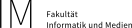
\includegraphics[scale=0.6]{anlagen/bilder/logos/IM-logo}
    \caption{Das Logo von Informatik und Medien }
\end{figure}

\begin{figure}[!t]
    \centering
    \includesvg[width=0.6\columnwidth]{anlagen/bilder/logos/IM-logo.svg}
    \caption{Das Logo von Informatik und Medien }
\end{figure}

Bedenken Sie bei allen Beschriftungen, egal ob Abbildungen, Tabellen oder Quelltexte, dass Sie, sofern diese nicht Ihrer eigenen Schaffenskraft entsprangen,
diese referenzieren. Im Beispiel der Tabelle \ref{tab:Beispieltabelle} sieht man, dass sich der Beschreibungstext direkt an der Tabelle von dem im Tabellenverzeichnis unterscheidet,
genau um den Punkt der Referenz.

\section{Methodik}

Im Methodik-Abschnitt (eine eigene Section) einer Arbeit stellen Sie die Methoden dar, die Sie verwendet haben oder vorhaben zu verwenden, um die Fragestellung zu beantworten. 
In diesem Abschnitt erläutern Sie, welche Methoden umgesetzt wurden (oder auch angedacht), um die Hypothesen zu testen und die Fallstudie durchzuführen. 
Welche Methoden für Ihre Arbeit geeignet sind, ist auch ein wesentlicher Punkt Ihres angestrebten Titels und somit ein zu bewertender Teil dieser Arbeit. 

\underline{Aber \textbf{mindestens} folgende Punkte}\\
Inhalt des ersten Kapitels (im Allgemeinen):
\begin{itemize}
    \item Thematische Einführung, umreißen des Themas \dots wo befinden wir uns?
    \item Herausstellen des Problems und warum es eines ist was gelöst werden sollte.
    \item Herausstellen der tatsächlichen Ziel-/Fragestellung, welche bearbeitet werden wird.
    \item Eine Abgrenzung was diese Arbeit ist und was sie nicht ist.
    \item Stand der Forschung \dots Was existiert bereits? Wie gut passt das auf das Problem?
    \begin{itemize}
        \item Referenzen mittels cite: \cite[S.~111]{jsch2011} \cite[S.~27f]{Tane2014}
    \end{itemize}
    \item Eine abgeleitete Methodik $\rightarrow$ basierend auf der Literatur und Ihrem Wissen: wie haben Sie nun vor Ihr Problem zu lösen? Vllt durch \cite{9429985}?
\end{itemize}


%##########################################################
% Zweites Kapitel
%##########################################################
%!TeX root = ./../Bachelorarbeit.tex

%##########################################################
% Inhalt
%##########################################################

\clearpage

\chapter{Theoretische Grundlagen}

\section{Emulation und Virtualisierung}

Um die Funktionsweise und Anwendung von QEMU zu verstehen müssen zuerst die
Begriffe der \textit{Virtualisierung} und \textit{Emulation} erklärt werden.
\newline
Virtualisierung ist eine Herangehensweise der Informationstechnik, welche
unterschiedliche Ressourcen in einer logischen Schicht zusammenfasst und somit
eine optimierte Auslastung
gewährleistet\cite{BSKompakt_Virt}.
Es handelt sich um ein Schlagwort, welches unterschiedliche Konzepte und
Techniken beschreibt und grob in zwei Bereiche unterteilt werden kann.
Die Virtualisierung von \textit{Software}, also die Verwaltung von
Software-Ressourcen wie Prozessen oder Betriebssystemen, sowie die
Virtualisierung von \textit{Hardware}, also die Verwaltung von
Hardware-Ressourcen, wie Recheneinheiten und
Speicher\cite{MasterkursVirtParaSys_Virt}.
% TODO: Hier auch noch etwas zur Emulation hinschreiben

\subsection{Virtualisierungstechniken}

In der Fachliteratur\cite{BSKompakt_Virt}\cite{BSGK_RBrause} unterscheidet man
mehrere Virtualisierungstechniken:
\begin{itemize}
    \item Partitionierung,
    \item Paravirtualisierung,
    \item vollständige Virtualisierung,
    \item Anwendungs- oder Softwarevirtualisierung,
    \item Betriebssystemvirtualisierung,
    \item Hardware-Virtualisierung.
\end{itemize}
Darüber hinaus gibt es noch andere Techniken wie
\textit{Netzwerkvirtualisierung}, welche aber in dieser Arbeit nicht betrachtet
werden.
Im Kontext von Systemen der \textbf{x86-Architektur} findet jede dieser
Techniken auf verschiedenen \textit{Privilegienstufen} statt.
Die x86-Architektur wird in dieser Arbeit als Standard Host-Plattform
angenommen und besitzt 4 verschiedene Stufen, auch Ringe
genannt\cite{BSKompakt_Syscall}.
\newline
Dabei sind vor allem \textit{Ring 0} (Kernelmodus), und \textit{Ring 3}
(Benutzermodus) von besonderer Bedeutung.
Im Kernelmodus läuft der Kernel des jeweiligen Betriebssystem. Alle Prozesse
auf dieser Stufe haben vollen Zugriff auf die Hardware\cite{BSKompakt_Syscall}.
\newline
Im Benutzermodus laufen alle übrigen Prozesse.
Prozesse dieser Stufe verfügen über geringere Privilegien und können nur über
\textit{Betriebssystemaufrufe} auf Funktionalitäten des Betriebssystemkernels
zugreifen\cite{BSKompakt_Syscall}.
% TODO: Was sind Syscalls?
Eine selbständige Erhöhung, bzw. Senkung, der Privilegienstufe ist nicht
möglich, was zur Sicherheit und Stabilität des gesamten Systems beiträgt.


Einige Virtualisierungstechniken nutzen einen \textit{Hypervisor}, manchmal
auch \ac{vmm} genannt.
Hypervisor werden in zwei Typen unterteilt.
\newline
Der sogenannte \textit{Typ-1-Hypervisor}, oder auch \textit{bare metal
Hypervisor}, läuft direkt auf der Systemhardware, ohne ein dazwischenliegendes
Betriebssystem.
Er übernimmt die Verteilung der Hardware-Ressourcen auf die unterschiedlichen
Prozesse und läuft im privilegierten Kernelmodus\cite{BSKompakt_Syscall}.
Ein Beispiel für einen Typ-1-Hypervisor ist das \ac{kvm} Modul des Linux
Kernels.
\newline
Ein \textit{Typ-2-Hypervisor}, auch \textit{hosted Hypervisor} genannt, läuft
als Anwendung in einem Host-Betriebssystem parallel zu anderen Prozessen im
weniger privilegierten Benutzermodus\cite{BSKompakt_Virt}.
Die Hardware-Ressourcen werden standardmäßig vom Host-Betriebssystem verwaltet
und der VM zur Verfügung gestellt.
Beispiele für Typ-2-Hypervisor sind Oracle Virtualbox und QEMU.

\begin{description}
    \item[Partitionierung]
        Das Konzept der \textit{Partitionierung} beschreibt die Aufteilung der
        Gesamtressourcen eines Systems auf verschiedene
        Teilsysteme\cite{BSKompakt_Virt}.
        Die Verwaltung findet hierbei direkt durch die Firmware des Systems
        statt.
        Es wird kein Hypervisor benötigt.
        Diese Technik findet vorrangig bei Großrechnern und Servern Anwendung.
        \clearpage
        % TODO: referenzieren im Text
        \begin{figure}[!htb]
            \centering
            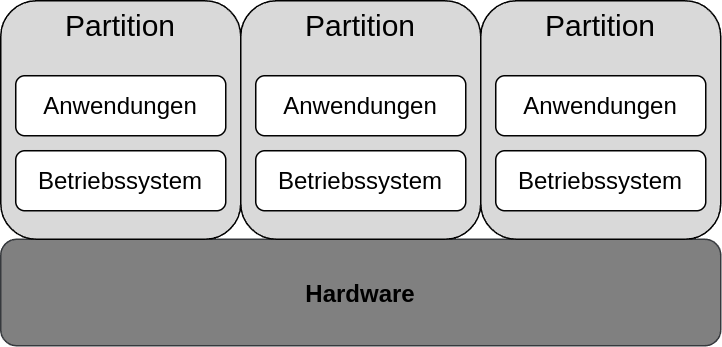
\includegraphics[width=0.5\textwidth]{anlagen/bilder/Partitionierung}
            \caption{Partitionierung der Hardware in individuelle
            Systeme\cite{PartAbb_BSKompakt}}
            \label{fig:Partitionierung}
        \end{figure}
    \item[Paravirtualisierung]
        Bei der \textit{Paravirtualisierung} wird ein Typ-1-Hypervisor genutzt,
        um die physischen Hardware-Ressourcen des Gesamtsystems zu verwalten.
        Dieser Hypervisor läuft im privilegierten Ring 0.
        Mithilfe dieser Technik können mehrere verschiedene Betriebssysteme auf
        diesem Hypervisor gleichzeitig nebeneinander ausgeführt
        werden\cite{BSGK_RBrause}.
        Die Kerne dieser Betriebssysteme werden im weniger privilegierten Ring
        1 ausgeführt und haben somit keinen direkten Zugriff auf die
        Hardware-Ressourcen.
        Anwendungen im Benutzermodus greifen daher zuerst mittels sogennanten
        \textit{Hypercalls} auf den Typ-1-Hypervisor zu, welcher dann die
        eigentlichen Systemaufrufe im Betriebssystem und den Zugriff auf die
        Hardware ausführt\cite{BSKompakt_Virt}.
    \item[vollständige Virtualisierung]
        Die \textit{vollständige Virtualisierung} beschreibt eine Technik, bei
        der ein Typ-2-Hypervisor ein gesamtes System inklusive aller Ressourcen
        und Schnittstellen (Netzwerkkarte, Laufwerke, etc.) virtualisiert
        bereitstellt\cite{BSKompakt_Virt}.
        Auf diesem virtuellen System wird ein Gast-Betriebssystem ausgeführt.
        Der Hypervisor läuft als Anwendung auf dem Host-Betriebssystem
        parallel zu anderen Prozessen.
        Alle privilegierten Systemaufrufe des Gast-Betriebssystems werden vom
        Hypervisor abgefangen und an das Host-Betriebssystem weitergeleitet.
    \item[Anwendungs-/Softwarevirtualisierung]
        Bei der \textit{Anwendungs-/Softwarevirtualisierung} werden einzelne
        Anwendungen in einer virtuellen Umgebung ausgeführt.
        Die virtuelle Umgebung befindet sich zwischen Host-Betriebssystem und
        Anwendung und stellt alle benötigten Funktionalitäten bereit.
        Sie läuft im weniger privilegierten Benutzermodus und hat keinen
        direkten Zugriff auf die Hardware-Ressourcen\cite{BSKompakt_Virt}.
        Bei dieser Technik kommt wie bei der Partitionierung kein Hypervisor
        zum Einsatz.
        Ein Beispiel für diese Technik ist die Java Virtual Machine in
        Verbindung mit der Java-Laufzeitumgebung.
    \item[Betriebssystemvirtualisierung]
        Die \textit{Betriebssystemvirtualisierung} funktioniert ähnlich zur
        Anwendungsvirtualisierung.
        Auf einem Host-Betriebssystem können mehrere, voneinander unabhängige,
        Systemumgebungen ausgeführt werden\cite{BSKompakt_Virt}.
        Diese werden \textit{Container} oder \textit{Jails} genannt.
        Im Unterschied zur Paravirtualisierung oder Partitionierung werden
        keine kompletten Gast-Betriebssysteme gestartet, sondern lediglich eine
        isolierte Laufzeitumgebung.
        Jeder Anwendung in einem spezifischen Container weiß nur von anderen
        Prozessen die im selben Container laufen.
        Sämtliche Zugriffe auf Hardware-Ressourcen werden vom
        Host-Betriebssystem verwaltet.
    \item[Hardware-Virtualisierung]
        Der Begriff der \textit{Hardware-Virtualisierung} beschreibt meist die
        x86-Befehlssatz-Erweiterungen von AMD und Intel, welche in aktuellen
        x86-kompatiblen Prozessoren zu finden sind\cite{BSKompakt_Virt}.
        Ziel dieser Erweiterungen ist die verbesserte Hardwareseitige
        Unterstützung für Hypervisor und virtuelle Maschinen auf
        x86-Plattformen.
        Es existieren Hersteller spezifische, untereinander inkompatible
        Lösungen, beispielsweise \textit{Intel VT} oder \textit{AMD-V}.
        Hardware-Virtualisierung wird in mancher Literatur aber auch synonym
        für Hardware-Emulation verwendet
        \cite{MasterkursVirtParaSys_Virt}.
        Der Unterschied zwischen Virtualisierung und Emulation wird
        anschließend erläutert.
\end{description}
% Put bit of space between text and image
\vspace{1ex}

% TODO: Im Text referenzieren
\begin{figure}[h]
    \begin{subfigure}{0.5\textwidth}
        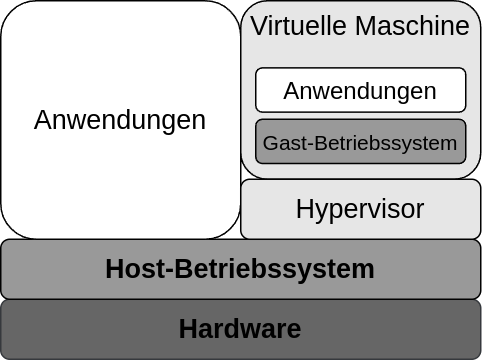
\includegraphics[width=0.9\linewidth]{anlagen/bilder/volle_Virtualisierung}
        \caption{Typ-2-Hypervisor lauft neben anderen Anwendungen auf
        Host-Betriebssystem}
        \label{fig:Volle_Virtualisierung}
    \end{subfigure}
    \hspace{1ex}
    \begin{subfigure}{0.5\textwidth}
        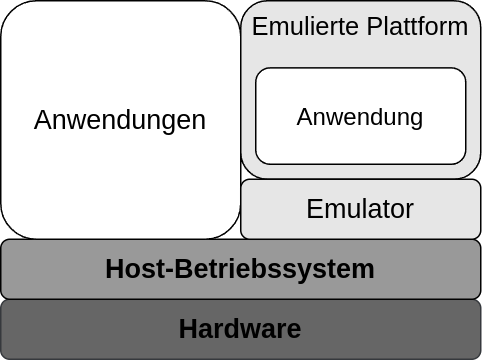
\includegraphics[width=0.9\linewidth]{anlagen/bilder/Software_Emulation}
        \caption{Software-Applikation läuft in emulierter Umgebung}
        \label{fig:Software_Emulation}
    \end{subfigure}
    \caption{Gegenüberstellung (a) vollständiger
    Virtualisierung\cite{VollVirtAbb_BSKompakt} und (b) Software
    Emulation\cite{SoftEmuAbb_BSKompakt}}
\end{figure}

\subsection{Hardware-Emulation}

Im Gegensatz zur Virtualisierung wird bei der Emulation die gesamte Hardware
eines Systems nachgebildet.
Man unterscheidet auch bei Emulation zwischen Hardware- und Software-Emulation.
Bei Software-Emulation werden die einzelnen Teile eines Systems wie
Maschinenbefehlssatz, Speicher und Schnittstellen virtuell in Software
nachgebildet\cite{BSKompakt_Virt}.
In dieser virtuellen Umgebung ist es möglich Softare auszuführen, welche
für eine andere Hardware-Plattform ausgelegt ist\cite{BSKompakt_Virt}.
Betriebssystemaufrufe und Zugriffe auf Peripherie werden in der
Emulationsumgebung behandelt.

% =============================================================================

\section{QEMU}

\textit{QEMU} ist ein generischer, quelloffener Maschinen Emulator und
Virtualisierer\cite{QemuAbout}.
Das Projekt wurde 2003 von Fabrice Bellard gestartet und läuft unter den
meisten Betriebssysteme wie Windows, Linux und MacOS.
QEMU emuliert die meisten gängigen Befehlssatzarchitekturen wie x86, ARM,
RISC-V, MIPS, und einige mehr\cite{WikiQemu}.
Die Emulationssoftware unterstützt unterschiedliche Modi.
Im Modus \textit{System Emulation} wird ein virtuelles Model einer Maschine
erzeugt, welches CPU, Speicher und Peripherie emuliert.
Auf der virtuellen Maschine kann anschließend ein Gast-Betriebssystem oder
andere unveränderte Anwendungssoftware ausgeführt werden.
\newline
Im Modus \textit{User Mode Emulation} können Anwendungen die für eine bestimmte
Befehlssatzarchitektur kompiliert wurden auf dem Host-Betriebssystem ausgeführt
werden.
\newline
QEMU kann sowohl als Kommandozeilenprogramm, als auch mit grafischer Oberfläche
ausgeführt werden.
Das QEMU Projekt stellt darüber hinaus verschiedene Kommandozeilen-Werkzeuge
zur Verfügung, zum Beispiel \texttt{qemu-img}, eine Anwendung mithilfe derer
ausführbare Betriebssystem-Images erstellt und bearbeitet werden können.

% TODO: Nähere Beschreibung von QEMU
%\subsection{Funktionsweise}
%User Mode vs Full System Emulation, Projektstruktur ?, TCG, Device und Board
% TODO: QOM und Device realization -> QEMU subsystem information
% TODO: Wie wird Board erstellt, in welcher beziehung stehen Board und GPIO controller
% TODO: Resettable Interface -> Verweis auf Mikrocontroller Reset?

% TODO-Anmerkung: Code morphing, Verbindung von VMM und Maschinenbefehl-Emulation
% Qemu als Grundlage von KVM

\subsection{Alternativen}
% TODO: Warum QEMU und nicht Renode / Virtual ARM -> Ausgereiftheit und non proprietär

Das QEMU Projekt besteht bereits seit einiger Zeit, daher kann eine hohe
Ausgereiftheit der Anwendung angenommen werden.
Darüber hinaus existieren bereits Implementationen für Mikrocontroller Modelle
der Produkt Familie STM32F4.
Es existieren einige Alternativen zu QEMU, davon sollen 2 kurz vorgestellt
werden.
Beide Alternativen erfüllen ähnliche Funktionen wie QEMU.
\begin{description}
    \item[Renode]
    \textit{Renode} ist ein quelloffenes Entwicklungs-Framework zur Simulation
    von Hardware Systemen inklusive CPU, Speicher, sowie dazugehöriger
    Peripherie\cite{RenodeAbout}.
    Ähnlich wie bei QEMU kann auch hier auf der emulierten Hardware
    unveränderte Anwendungssoftware ausgeführt werden.
    \item[ARM Virtual Hardware]
    Bei \textit{ARM Virtual Hardware} handelt es sich um ein proprietäres
    Emulations Werkzeug für ARM basierte Systeme, welches in der Cloud
        ausgeführt werden kann\cite{ArmVirtualHwAbout}.
\end{description}

% =============================================================================

\section{Mikrocontroller und Mikroprozessoren}

In eingebetteten Systemen findet man oftmals sogenannte Mikrocontroller, welche
die Steuerung verschiedener Funktionalitäten übernehmen.
Ein Mikrocontroller besteht in der Regel aus mehreren Komponenten.
Einem Mikroprozessor für die Abarbeitung des Programmcodes, Arbeits- und
Programmspeicher, Peripherie für Kommunikation oder Ein-/Ausgabe, und
Taktgeneratoren als interne Takt- und Synchronisierungsquelle.
Alle Komponenten sind mittels eines Systembuses miteinander
vernetzt\cite{DefGuideCM34_JYiu}.
Der Mikroprozessor nimmt hierbei meist nur einen geringen Platz der Chipfläche
ein.
Bei komplexen Hardware-Designs spricht man auch von einem \ac{soc}.
\newline % TODO: Quelle! -> Nicht ganz korrekt -> SoC kein Überbegriff
Im Bereich der eingebetteten Systeme sind ARM Mikroprozessoren weit verbreitet.
ARM selbst produziert keine Mikrocontroller.
Sie entwickeln die Mikroprozessoren und verkaufen die Lizenzen zur Produktion
an externe Hersteller, welche sie anschließend in ihre Mikrocontroller-Designs
integrieren.
\newline
Die ARM Mikroprozessor-Familien werden in 3 verschiedene Familien unterteilt.
\textit{Cortex-M}, \textit{Cortex-R} und \textit{Cortex-A} Mikroprozessoren.

% TODO: Welche Familien 32 bzw 64 Bit, Befehlssatzarchitektur, CISC/RISC
% Multicore ? Multi threaded Applikationen
\begin{description}
    \item[Cortex-M]
    Die \textit{Cortex-M} Familie ist eine Familie von 32-bit Mikroprozessoren,
    welche erstmals 2005 veröffentlicht wurden\cite{DefGuideCM34_JYiu}.
    Die Prozessor-Familie ist für eine besonders breite Fläche an
    Elektronischen-Anwendungen geeignet, von Mobiltelefonen bis hin zur
    Integration in Automobil-Systeme.
    Innerhalb der Cortex-M Familie gibt es unterschiedliche Prozessor-Typen,
    beispielsweise Cortex-M0, Cortex-M0+, Cortex-M1, Cortex-M3 und
    Cortex-M4\cite{DefGuideCM34_JYiu}.
    Für diese Arbeit werden Mikrocontroller betrachtet, welche Mikroprozessoren
    des Typs Cortex-M3 oder Cortex-M4 integrieren.
    Da es nur geringe Unterschiede zwischen Cortex-M3 und M4 gibt, werden diese
    im weiteren Verlauf als synonym betrachtet.
    \item[Cortex-R] 
    Mikroprozessoren der Familie \textit{Cortex-R} sind für spezielle, komplexe
    Anwendungen mit Echtzeit-Anforderungen ausgelegt.
    Prozessoren dieser Familie werden dort eingesetzt, wo hohe Zuverlässigkeit
    und Determinismus benötigt werden, beispielsweise bei
    Festplattencontrollern oder Automobil-Systemen\cite{DefGuideCM34_JYiu}.
    \item[Cortex-A] 
    Die \textit{Cortex-A} Mikroprozessor Familie sind für rechenintensive,
    \textit{high-end} Applikationen ausgelegt.
    Meist läuft auf einem Cortex-A Mikroprozessor ein vollwertiges
    Betriebssystem, mit Unterstützung für virtualisierte Speichertechniken,
    sowie einer Speicherverwaltungseinheit\cite{DefGuideCM34_JYiu}.
    % TODO: Quelle
    Beispiele hierfür sind moderne Smartphones mit \textbf{Qualcomm Snapdragon}
    oder \textbf{Apple Silicon} Prozessoren.
\end{description}

% TODO: "Peripherie des STM32F4" besser Titel?
% Aufbau eines Peripherie Moduls, welche Register, wie Addresierbar, MMIO ??
\subsection{UART Protokoll}

\ac{uart}, sowie die Erweiterung \ac{usart}, bezeichnen elektronische
Schaltungen für Sender und Empfänger asynchroner, sowie synchroner
Datenübertragung\cite{Digitec_WGehrke_MWinzker}.
U(S)ART-Schnittstellen werden zum Senden und Empfangen serieller Daten benutzt.
Konkrete Schnittstellen sind beispielsweise \textbf{RS-232} oder
\textbf{EIA-485/RS-485}.
Während im Bereich der Heimcomputer durch die Einführung leistungsfähigerer
Übertragungsmethoden, wie Ethernet oder WLAN, die serielle Datenübertragung an
Bedeutung verloren hat, ist sie im Bereich der Mikrocontroller und eingebetter
Systeme weiterhin weit verbreitet\cite{Digitec_WGehrke_MWinzker}.
% TODO: Grobe Erklärung einer Schaltung, Verbindungsaufbau und Datenpaket
% Was ist Baudrate, wozu kann UART in Mikrocontrollern genutzt werden?

\subsection{GPIO}
\label{sec:theo-basics-gpio}
% TODO: Wie viele GPIOs (Ports) im Soc??
% TODO: MMIO

Ein \ac{gpio}-Pin ist ein elektronischer Kontakt, welcher durch Software als
Eingabe- oder Ausgabe-Kontakt konfiguriert werden
kann\cite{Digitec_WGehrke_MWinzker}.
Wie der Name schon sagt haben GPIO-Pins keine feste, vordefinierte Funktion.
% TODO: Erklärung Register für Peripherie, siehe oben.
% Erklärung Konfiguration von GPIO Registern
Die Konfiguration der Pins erfolgt durch das Setzen und Löschen sogenannter
Kontroll-Register.

% =============================================================================

\section{Softwareentwicklungsprozess für eingebettete Systeme}

Um eine Applikation für einen Mikrocontroller zu entwickeln und anschließend
auf einem realen System zu testen müssen mehrere Schritte durchlaufen werden.
Im folgenden sollen die Softwaretechnischen Rahmenbedingungen für die
Mikrocontroller-Entwicklung kurz vorgestellt und erläutert werden.

% TODO: Was ist CMSIS, wofür wird es gebraucht, wer hat es eingeführt
% TODO: HAL was ist es, wie eingesetzt?
% TODO: Middleware
\subsection{Softwaretechnische Grundlagen}

% TODO: Quelle
Die de-facto Standard-Programmiersprachen im Umfeld der eingebetteten Systeme
sind \textit{C} und \textit{C++}.
Darüber hinaus werden auch \textit{Rust}, \textit{Java} oder
\textit{Javascript} genutzt.
\newline
Software Applikationen für eingebettete Systeme reichen von sogenannten
\textit{Bare Metal} Applikationen, über Applikationen mit integriertem
\textit{\ac{rtos}} bis hin zu Anwendungen die auf einem \enquote{normalen}
Mehrbenutzer-Betriebssystem laufen.
\newline
Bare Metal bedeutet, dass der Zugriff auf Hardware-Ressourcen und
Peripherie-Schnittstellen nicht von einer Abstraktions-Schicht des
Betriebssystem verwaltet wird.
Er erfolgt direkt über die Anwendungssoftware.
Somit liegen dynamische Speicherallokation oder auch die Verwaltung
konkurrenter Zugriffe auf Peripherie-Schnittstellen in der Verantwortung des
Softwareentwicklers.
\newline
Ein Echtzeitbetriebssystem ermöglicht eine konkurrente Ausführung mehrere
Aufgaben bei gleichzeitiger Einhaltung fester Zeitbedingungen.
Maßgebend für ein Echtzeitbetriebssystem ist dabei nicht die Schnelligkeit
einer Reaktion auf ein Ereignis, sondern die Einhaltung einer fest definierten
Zeitschranke\footnotemark[1]\cite{BSKompakt_GrundlagenBs}.
\newline
Mit steigender Rechenleistung und Verfügbarkeit von Speicher im Umfeld der
eingebetteten Systeme steigen auch die Anforderungen an die parallele,
beziehungsweise konkurrente, Abbarbeitung einer Vielzahl an Aufgaben.
Eine Alternative zu herkömmlichen Echtzeitbetriebssystemen ist \textit{Embedded
Linux}.
Es handelt sich um ein modifiziertes Betriebssystem auf Basis des
\textit{Linux-Kernels}.
Die vergleichsweise einfache Anpassbarkeit des Linux Kernels und die hohe
Verfügbarkeit an kompatiblen Hardware-Plattformen ermöglichen eine Vielzahl an
Einsatzmöglichkeiten\cite{UbuntuBlogEmbeddedLinux}.

% Deadline Footnote
\footnotetext[1]{englisch: \textit{Deadline}}

\subsection{Interprozesskommunikation}

Bei \ac{ipc} handelt es sich um eine Form der Informationsübertragung zischen
unterschiedlichen Prozessen eines Betriebssystems.
% TODO: IPC erklären für Code Dive Integration
% TODO: Nanomsg und bekannte alternativen


%##########################################################
% Drittes Kapitel
%##########################################################
%!TeX root = ./../Bachelorarbeit.tex

%##########################################################
% Inhalt
%##########################################################

\clearpage
\chapter{Konzeption}

\section{Auswahl der Peripherie}
\label{sec:concept-periphery-selection}

Für diese Arbeit wurde das \textit{\ac{gpio}} und das
\textit{\ac{uart}}-Peripheriemodul für Tests und Implementierung ausgewählt.
Beide Schnittstellen sind für eingebettete Systeme unerlässlich und können für
verschiedenste Anwendungen eingesetzt werden.
\newline
UART wurde ausgewählt, da der Aufwand der Integration bereits in QEMU
bestehender Schnittstellen bewertet werden soll.
Es existiert bereits eine Implementation eines UART Controllers für einen
Mikrocontroller der STM32F2-Familie.
Da Mikrocontroller Modelle der STM32F2 und STM32F4 Familien Pin-kompatibel
sind, sollte die bestehende Implementation des UART Controllers ebenfalls
für den STM32F429 SoC verwendet werden können.
Darüber hinaus ist die Funktionalität von UART im Vergleich zu anderen
seriellen Schnittstellen einfacher zu testen.
Es können Funktionen wie ARM's \textit{Semihosting} verwendet werden, um
beispielsweise durch UART übertragene Zeichen in der Kommandozeile auszugeben.
Dies verringert die Komplexität der Testprogramme, da keine speziellen
Änderungen für die jeweilige Testumgebung (QEMU oder echte Hardware) erfordlich
sind.
\newline
Die GPIO Schnittstelle wurde für eine neue, eigenständige Implementierung in
QEMU ausgewählt.
Sie weist eine vergleichsweise geringe Komplexität auf.
Testprogramme für die GPIO Funktionalität sollten ebenfalls ohne Anpassungen
sowohl in QEMU, als auch auf echter Hardware laufen.
In QEMU Version 9.0 existiert bereits eine Integration für einen
Mikrocontroller der STM32L4-Familie.
Das GPIO-Peripheriemodul der STM32L4-Familie ist allerdings nicht kompatibel
zum GPIO-Peripheriemodul der STM32F4-Familie.
Es verfügt über eine andere Anzahl an Peripherie Registern, mit anderen
Funktionalitäten.
Die Implementierung kann daher nur als Orientierung dienen und muss
entsprechend angepasst werden.

% TODO: Entwicklungsumgebung
% TODO: Unterschied Simulation und Emulation
\section{QEMU Erweiterung}

QEMU unterscheidet bei der Emulation von ARM Systemen zwischen Maschinen und
\ac{cpu}'s.
Die Maschine ist in der Regel ein spezielles Entwicklungsboard eines
Herstellers, welches einen \ac{soc} auf einer Leiterplatte integriert, zum
Beispiel das STM32F429-Discovery\cite{Stm32F429DiscoveryBoard} oder das
Olimex-STM32-E407\cite{OlimexStm32E407Board}.
\newline
In QEMU werden Maschine und SoC meist getrennt implementiert.
Die Maschine, bzw. das Entwicklungsboard, agiert dabei als Container für den
SoC.
Die meisten Funktionalitäten, sowie die Peripherie, werden im SoC
implementiert und der Maschine zur Verfügung gestellt.
Die CPU ist für die meisten \acp{soc} festgesetzt, da auf der echten Hardware
ebenfalls standardmäßig nur eine CPU zur Anwendung kommt.
Die CPU Architektur des STM32F429 Mikrocontrollers, \textit{Cortex-M4F} kann
vollständig in QEMU emuliert werden.
Beide der folgenden Ansätze sollen die CPU Emulation nutzen und um bestimmte
Peripherien erweitern.

% TODO: EXTI benutzen?
\subsection{QEMU Device Implementierung} \label{konzept-qemu-dev}

Zunächst soll untersucht werden, wie eine Maschine und der dazugehörige SoC
direkt in QEMU integriert werden kann.
Das QEMU Projekt ist bereits über 20 Jahre alt und verfügt über diverse
\acp{api}.
Diese sollen genutzt werden um das Projekt durch den STM32F429-\ac{soc} zu
erweitern.
Desweiteren soll eine Maschine integriert werden welche den \ac{soc}
implementiert.
Der grobe Ablauf dieser Erweiterung besteht also aus folgenden Abschnitten:
\begin{enumerate}
    \item Hinzufügen neuer Build-System Konfiguration für \ac{soc},
    \item Implementierung des STM32F429-\ac{soc},
    % TODO: Spezifiziere welche Peripherie
    \item Integration bestehender Peripherie in \ac{soc},
    \item Hinzufügen neuer Build-System Konfiguration für GPIO-Peripherie
    \item Implementierung der neuen Peripherie und Integration in \ac{soc}
\end{enumerate}
Die Adressen der Peripherie müssen dem Technischen-Referenzwerk des
STM32F429-Mikrocontrollers entnommen werden.
Die Funktionsweise und Konfiguration der Peripherie-Register sind dort
ebenfalls beschrieben.
\begin{figure}[!htb]
    \centering
    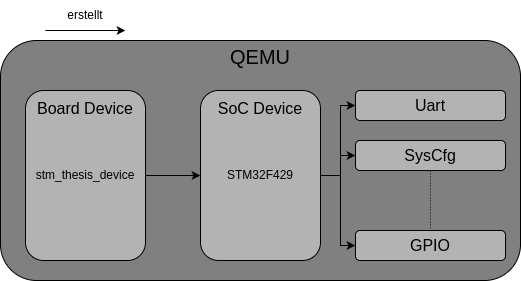
\includegraphics[width=0.7\textwidth]{anlagen/bilder/Qemu_Device}
    \caption{Grobe Skizzierung der Interaktion zwischen Maschine, \ac{soc} und Peripherie}
    \label{fig:QemuDeviceErweiterung}
\end{figure}


% TODO: Kompilieren von EDI Repo mit libnanomsg
\subsection{External Device Interface Implementierung}

Im zweiten Ansatz soll ein weiteres Konzept für die Integration neuer
\ac{soc}'s in QEMU vorgestellt werden.
Bei dieser Methode wird die Implementierung der Peripherie in externe Prozesse
verlagert.
Die Unterscheidung zwischen CPU und Maschine besteht zwar auch bei diesem
Ansatz, allerdings ist der Funktionsumfang der Maschine stark reduziert, da sie
keine Peripherie direkt über den \ac{soc} integriert.
Die relevanten Schnittstellen laufen jeweils gekapselt in einem separaten
Prozess und kommunizieren mittels \ac{ipc} mit der QEMU-Anwendung.
\begin{figure}[!htb]
    \centering
    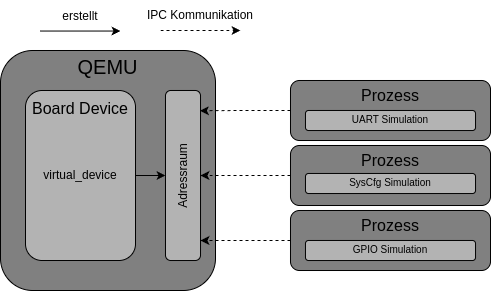
\includegraphics[width=0.7\textwidth]{anlagen/bilder/Qemu_external_device}
    \caption{Grobe Skizzierung der Interaktion zwischen QEMU und externen Prozessen}
    \label{fig:QemuExternalDeviceErweiterung}
\end{figure}
Dies ermöglicht eine unabhängige Implementierung von Peripherie und \ac{soc}.
Die Interprozesskommunikation wird mittels einer externen Bibliothek
realisiert, welche in die QEMU Anwendung integriert werden muss.
Im Gegensatz zum ersten Ansatz muss nicht für jeden neuen Mikrocontroller eine
separate Maschine mitsamt \ac{cpu} implementiert werden.
Stattdessen reicht eine generische Maschine welche den jeweiligen \ac{cpu}-Typ
integriert.
Um die Komplexität gering zu halten soll nur die im STM32F429-\ac{soc}
verwendete \ac{cpu} benutzt werden.
Die Verbindung von QEMU-Emulation und den separaten Prozessen erfolgt bei Start
der QEMU-Anwendung.
Dort können einzelne Devices oder eine Gruppe von Devices mit einer
spezifischen Adresse im Adressraum des \ac{soc} verbunden werden.

% TODO: Was sind Voraussetzungen für Programm?? -> zusätzlich zu Startup auch Tick und anderes
% TODO: Wieso kein StmCube und/oder Keil MDK ARM
% TODO: Wieso meson, wie funktioniert meson mit cross compile
% TODO: Wie sind Testaufbauten geplant? -> Richtige Testaufbauten dann in Implementaiton
% TODO: Projektaufbau
% TODO: Vergleichende tests qemu und hardware
% TODO: Bei gpio test Programm -> Falls timer nicht abstrahiert einfach loop zählen lassen
\section{Testprogramme und Teststrategie}

Um die korrekte Funktionsweise der Peripherie und \ac{soc} Implementierungen zu
testen sollen verschiedene Testprogramme entwickelt werden.
Diese Testprogramme werden anschließend sowohl in QEMU als auch auf realer
Hardware ausgeführt.
Da bei allen Ansätzen der gleiche \ac{soc} mit gleicher \ac{cpu} eingesetzt
wird reicht es die Tests auf die jeweilige Peripherie zu beschränken.
Während der Ausführung können unterschiedliche Verhalten in der Software für
emulierte und reale Umgebung auftreten.
Um diese möglichst gering zu halten sollen die Testprogramme eine möglichst
geringe Komplexität aufweisen.
\newline
Für die Entwicklung der Tests sollen ausschließlich die notwendigsten externen
Bibliotheken genutzt und konfiguriert werden.
Dies umfasst die STM-\textit{\ac{hal}}, für Programmierung und Konfiguration
der Peripherie.
Zur Konfiguration der der \ac{cpu} spezifischen
Einstellungen soll das \textit{\ac{cmsis}} verwendet werden.
Die eigentliche Testanwendung wird dann in \textit{C} programmiert.
Für die Testprojekte wird das Build-System \textit{Meson} verwendet, da dies
auch im QEMU Projekt zum Einsatz kommt und somit keine erneute Umgewöhnung
erfordert.


%##########################################################
% Viertes Kapitel
%##########################################################
%!TeX root = ./../Bachelorarbeit.tex

%##########################################################
% Inhalt
%##########################################################

\clearpage

\chapter{Implementation}

\section{QEMU Device Erweiterung}

Wie in \ref{konzept-qemu-dev} beschrieben werden Peripherie und Mikrocontroller
in QEMU durch verschiedene \acp{api} integriert.
QEMU implementiert mithilfe der \ac{qom}- und \ac{qdev}-\acp{api} einen
Objektorientierten Ansatz.
Da C keine Objektorientierte Programmiersprache ist und nur ein vergleichsweise
minimales Typsystem unterstützt werden in QEMU viele dieser Konzepte mittels
Makro-Programmierung\footnotemark[1] realisiert.
\newline
Jede Maschine und jede Peripherie in QEMU ist ein Objekt einer Klasse.
Moderne Klassen in QEMU sollten von der \texttt{TYPE\_SYS\_BUS\_DEVICE} Klasse
erben.
Vom Typ \texttt{TYPE\_SYS\_BUS\_DEVICE} erbende Objekte werden im Falle eines
Reset-Events automatisch zurückgesetzt.
Das Reset-Event und Resettable-Interface werden in Kapitel
\ref{sec:impl-qemu-reset} erklärt.
Die Details der Instanziierung einer Klasse werden in Kapitel
\ref{sec:impl-qemu-device-build-obj} erläutert.
\newline
Nach Aufstart von QEMU wird als Erstes die Maschine erzeugt.
Welche Maschine gestartet werden soll wird durch den Kommandozeilenbefehl
\texttt{-machine/-M} ausgewählt.
Die Maschine erstellt \ac{cpu} und \ac{soc}, welcher anschließend für die
Realisierung der Peripherie zuständig ist.
So ensteht eine Baum-Hierarchie, welche in QEMU auch \enquote{QOM-tree} genannt
wird.
Im QOM-tree sind alle Objekte einer Maschine repräsentiert.
\newline
Im ersten Schritt werden die Quelldateien dem Build-System hinzugefügt.
Für eine bessere Abgrenzung wird die neue Maschine
\texttt{stm32f429-thesis-device} erstellt, welche das \enquote{Testboard} in
QEMU darstellen soll.

\subsection{Build-Konfiguration und Objekt Erstellung}
\label{sec:impl-qemu-device-build-obj}

Um eine neue ARM Maschine zu registrieren muss die Konfiguration der
\textbf{Kconfig}\footnotemark[2] Datei im ARM Verzeichnis angepasst werden.
QEMU erstellt für die Emulation jeder unterstützten Architektur ein
individuelles Binary, beispielsweise \texttt{qemu-system-arm} oder
\texttt{qemu-system-x86}.
Mittels Kconfig und Meson wird sichergestellt das Quelldateien nur für die
vorgesehenen Architekturen in das jeweilige Programm gelinkt werden.
Ein Kconfig-Eintrag besteht aus der Definition selbst und einer variablen
Anzahl an Modulen die eingebunden werden.

% Makro-Programmierung Footnote
\footnotetext[1]{In C werden Textmakros vor der Übersetzung vom
Präprozessor ersetzt.}
% Kconfig Erklärung Footnote
\footnotetext[2]{Kconfig entstandt ursprünglich im Linux-Kernel Projekt und
wird in QEMU zur Verwaltung der Abhängigkeiten verwendet\cite{QemuDocsKconfig}.}

\begin{minipage}{\linewidth}
\lstinputlisting[language=,numbers=none,
                label={lst:qemu-kconfig},
                linerange={157-162,467-478},
                caption=ARM Kconfig Konfiguration von Maschine und \ac{soc}]
                {anlagen/qemu-device/KConfig.config}
\end{minipage}

Für die Einbindung des Mikrocontrollers werden in \ref{lst:qemu-kconfig} die
Konfigurationen für den \ac{soc} und die Maschine hinzugefügt.
Die Maschine benötigt das \ac{tcg} und ARM Modul.
Mit \texttt{select} wird der STM32F429-\ac{soc} der Maschine hinzugefügt und
beim Build-System registriert.
In der Konfiguration des \ac{soc} wird anschließend ausgewählt, welche
Peripherie und welcher Mikroprozessor verwendet werden soll.
Im Falle des STM32F429 ist ein ARM Cortex-M4 Mikroprozessor verbaut, welcher
auf der ARM-V7M Architektur basiert.
Als Vorlage für die Maschine wurde das bereits in QEMU implementierte
\textbf{olimex-stm32-h405} Entwicklungsboard verwendet\cite{QemuOlimexBoard}.
Die Grundlage für den STM32F429-\ac{soc} bildet der vom Olimex-Board verwendete
STM32F405-\ac{soc}\cite{QemuStmF405Soc}.
\newline
In \ref{lst:qemu-soc-header} wird der State für den STM32F429-\ac{soc} als
\texttt{struct} deklariert.
Hier erfolgt auch die Deklaration des STM32F429-\ac{soc} Typs.
Er implementiert die unterschiedlichen Peripherie-Devices, Speicherregionen,
sowie System- und Referenz Takt.
Für STM32F4 und STM32F2 Mikrocontroller existieren bereits unterschiedliche
Peripherien.
In der QEMU Dokumentation wird beschrieben, dass die Produktfamilien STM32F4
und STM32F2 Pin kompatibel sind.
Es können also auch Peripherie Implementationen für Mikrocontroller der
STM32F2-Familie verwendet werden.
Die Peripherie wird später während der \ac{soc}-Realisierung als \enquote{QEMU
Device} erstellt und dem QOM-tree hinzugefügt.
\newline
Tabelle \ref{tab:stm32-memory} zeigt die verschiedenen Speichertypen des
STM32F429-\ac{soc}.
Die Daten sind im STM32-\ac{trm} Sektion 3.4 für Flash-Speicher und Sektion
2.3.1 für \ac{sram} und \ac{ccm} definiert\cite{Stm32F4Trm}.
Die Speicherregionen werden ebenfalls während der Initialisierung des \ac{soc}
realisiert.

\begin{table}[h!]
    \centering
    \caption{Speichertypen mit Größe und Startadresse im 32-Bit-Adressraum}
    \label{tab:stm32-memory}
    \begin{tabular}{||P{3cm}|P{5cm}|P{4cm}||}
        \hline
        \textbf{Speichertyp} & \textbf{Speichergröße in KB} & \textbf{Startadresse} \\
        \hline
        \hline
        \hspace{0.8cm}
        Flash & 2048 & 0x0800 0000 \\
        \hline
        \hspace{0.8cm}
        \ac{sram} & 256 & 0x2000 0000 \\
        \hline
        \hspace{0.8cm}
        \ac{ccm} & 64 & 0x1000 0000 \\
        \hline
    \end{tabular}
\end{table}

Um die Maschine in der Kommandozeilenanwendung auszuwählen, muss diese
allerdings erst noch als statischer Typ registriert werden.
Die Registrierung einer Maschine unterscheidet sich leicht von der eines
Devices.
In \ref{lst:qemu-machine-init} erfolgt die Registrierung der neuen Maschine.
Das Makro \texttt{DEFINE\_MACHINE} registriert die Maschine als statischen Typ.
Anders als bei einem Device ist die Basisklasse einer Maschine
\texttt{MACHINE\_TYPE}.
Die Methode \texttt{stm32\_f429\_thesis\_machine\_init} ist verantwortlich für
die \enquote{oberflächliche} Initialisierung der Maschine.
Falls vorhanden können hier Argumente verarbeitet werden, die bei Aufstart von
QEMU über die Kommandozeile Argumente übergeben wurden.
Des Weiteren enthält sie die Beschreibung der Maschine, sowie die konkrete
Initialisierung durch die \texttt{stm32\_f429\_thesis\_init} Methode.
In der konkreten Initialisierung werden Mikroprozessor und \ac{soc} erstellt.
Da alle STM32F429 Mikrocontroller den Cortex-M4 Mikroprozessor wird nur dieser
erlaubt.
Sowohl für Maschinen als auch normale Devices existieren eine Methode zur
Initialisierung der Klasse, und eine Methode zur Initialisierung des Objekts.
Eine \texttt{class\_init} Methode wird immer vor Aufruf der Objekt
Initialisierung ausgeführt.

\begin{minipage}{\linewidth}
\lstinputlisting[language=c,numbers=none,
                label={lst:qemu-machine-init},
                linerange={36-51},
                caption=Initialisierung und Registrierung der STM32F429-thesis Maschine]
                {anlagen/qemu-device/stm32f429_thesis.c}
\end{minipage}

\subsection{GPIO-Peripherie des STM32F429}

Wie in \ref{sec:concept-periphery-selection} erwähnt soll das \ac{gpio}-Module
implementiert werden.
Die Konfiguration des Build-Systems erfolgt analog zur Implementation der
Maschine und des \ac{soc}.
Es müssen die Kconfig und Meson Konfiguration im \ac{gpio}-Peripherie Verzeichnis
angepasst werden.
Jeder \ac{gpio} Port wird als ein eigenständiges Device modelliert.
In \ref{lst:qemu-gpio-header} wird der State für das \ac{gpio} Device erneut als
\texttt{struct} deklariert.
Alle Register sind 32-Bit breit und können als vorzeichenlose 32-Bit Ganzzahlen
dargestellt werden.
\newline
Aufgrund hoher Komplexität und fehlender Peripherie des STM32F429 in QEMU
können nicht alle Funktionalitäten des \ac{gpio} Moduls abgebildet werden.
Die \enquote{alternative Funktion}\footnotemark[3] und die Regulierung der
Eingabe-/Ausgabe-Frequenz eines \ac{gpio} Pins werden nicht unterstützt.
Es fehlen beispielsweise Unterstützung für Ethernet- und \ac{can}, sowie die
Implementation der \ac{rcc}-Peripherie.
% Alternate Function Footnote
\footnotetext[3]{english: alternate function}
In \ref{lst:qemu-gpio-memops} wird die Speicherregion während der
Initialisierung des Objekts initialisiert und dem Systembus bekannt gemacht.
Auf dem Systembus werden die meisten Peripherie Devices registriert.
In QEMU können jeder Speicherregion bestimmte Eigenschaften zugewiesen werden.
Dies erfolgt über ein Objekt des Typs \texttt{MemoryRegionOps}.
In diesem Objekt können verschiedene Eigenschaften bestimmt werden.
Lese- und Schreibzugriff auf die \ac{mmio}-Region (bzw. die Register) werden
über die Funktionen \texttt{stm32f429\_gpio\_read} und
\texttt{stm32f429\_gpio\_write} realisiert.
Diese werden als \enquote{Callbacks} registriert.
Es wird ebenfalls die Byte-Reihenfolge, sowie die erlaubte Größe eines Lese-
oder Schreibzugriffs festgelegt.
\newline
Um die Komplexität der \enquote{write}-Funktion zu verringern wird nur
ein 4 Byte (32-Bit) Zugriff erlaubt.
Damit werden umständliche und fehleranfällige Bit-Manipulationen unnötig.
Jedes Register des \ac{gpio}-Moduls hat einen individuellen Offset.
Dieser Offset kann in Sektion 8.4 des \ac{trm} für jedes Register nachgelesen
werden\cite{Stm32F4Trm}.
Sowohl der write- als auch der read-Funktion wird ein Offset Wert als Parameter
übergeben.
Der Offset in die \ac{mmio}-Speicherregion errechnet sich nach der simplen Formel
\ref{eq:qemu-gpio-mmio-offset}.
In beiden Funktionen kann dann mittels einer \texttt{switch-case} Anweisung des
\texttt{Offset\_\ac{mmio}} der Zugriff auf das jeweilige Register bestimmt
werden.
Bei einem Schreibzugriff wird der Funktion darüber hinaus noch ein Schreibwert
übergeben, der in das Register geschrieben wird.
\begin{equation}
    Offset_{\ac{mmio}} = Basisadresse_{\ac{mmio}} + Offset_{Parameter}
    \label{eq:qemu-gpio-mmio-offset}
\end{equation}
Sowohl bei lesendem, als auch bei schreibendem Zugriff kann je nach Register
der Status des \texttt{LCKR}-Registers aktualisiert werden.

Das \ac{gpio}-Modul des STM32F429 kann durch eine bestimme Sequenz an Schreib- und
Lesezugriffen auf das \texttt{LCKR}-Register die
Konfigurationsregister\footnotemark[4] \enquote{einfrieren}.
Diese Sequenz kann der Sektion 8.4.8 des \ac{trm} entnommen werden\cite{Stm32F4Trm}.
Der Pseudocode \ref{alg:qemu-device-lckr} erläutert den groben Ablauf der
Lock-Sequenz Implementation im \ac{gpio} State.
Die Sequenz besteht aus drei Schreib- und einem Lesezugriff, welche
nacheinander ausgeführt werden müssen.
Bei jedem Schreibzugriff müssen Bits 0 bis 16 gleichzeitig gesetzt werden.
Ein Zugriff auf das \texttt{LCKR}-Register ist daher nur als 32 Bit Zugriff
möglich.
Wird die Reihenfolge der Zugriffe nicht eingehalten, wird die Sequenz
abgebrochen und muss von neuem gestartet werden.
Nach Schritt 4, dem Lesezugriff, wird die Lock-Konfiguration angewendet.
Für jedes gesetzte Bit der Lock-Konfiguration\footnotemark[5] können die
korrespondierenden Bits in den Konfigurationsregistern nicht mehr geändert
werden.
\begin{algorithm}
    \floatname{algorithm}{Algorithmus}
    \caption{\texttt{LCKR}-Register Lock-Sequenz der Konfigurationsregister der
            \ac{gpio} Pins}
    \label{alg:qemu-device-lckr}
    \begin{algorithmic}[1]
        \State \textbf{Write} $lckr$ \gets \textbf{Set} $lckr[16]$ + $lckr[0..15]$
        \Comment{lckr[16] ist der Lock Schlüssel}
        \State \textbf{Write} $lckr$ \gets \textbf{Reset} $lckr[16]$ + $lckr[0..15]$
        \State \textbf{Write} $lckr$ \gets \textbf{Set} $lckr[16]$ + $lckr[0..15]$
        \State \textbf{Read} $lckr$
    \end{algorithmic}
\end{algorithm}

Die Lock-Konfiguration kann bis zum \textit{Reset} des Mikrocontrollers
nicht mehr geändert werden.
% Konfigurationsregister Footnote
\footnotetext[4]{Die Konfigurationsregister sind \texttt{MODER},
\texttt{OTYPER}, \texttt{PUPDR} und \texttt{OSPEEDR}.}
% LCKR Konfiguration Footnote
\footnotetext[5]{Die Lock-Konfiguration der \ac{gpio} Pins ist in den Bits 0
bis 15 des \texttt{LCKR} Registers enthalten.}
\newline
Die Implementation in QEMU wird in \ref{lst:qemu-gpio-lckr-write} exemplarisch
für den ersten Schritt der Sequenz dargestellt.
Bei einem Lese- oder Schreibzugriff auf das \texttt{LCKR}-Register wird die
Funktion \texttt{update\_lckr} ausgeführt.
Die Funktion erhält einen Zeiger auf den \ac{gpio}-State, den Wert, der in das
Register geschrieben werden soll und ein Flag welches anzeigt, ob es sich um
einen Lese- oder Schreibzugriff handelt.
Bei einem Lesezugriff wird als Wert das aktuelle \texttt{LCKR}-Register
übergeben.
Sind die Bedingungen für den ersten Schritt der Sequenz erfüllt, wird der Wert
des \texttt{LCKR}-Registers aktualisiert.
Der \texttt{lock\_state} wird auf den nächsten Schritt der Sequenz gesetzt.
Verändert sich während eines Schrittes der Lock-Sequenz die Konfiguration der
Port-Bits, wird die Sequenz abgebrochen und muss erneut gestartet werden.

% Code manuell reinschreiben, da wir nicht die ganze Funktion zeigen wollen und
\begin{minipage}{\linewidth}
\begin{lstlisting}[language=c,numbers=none,
                label={lst:qemu-gpio-lckr-write},
                caption=\texttt{update\_lckr} Funktion mit Implementation des
                    ersten Schreibzugriffes auf das \texttt{LCKR}-Registers]
    switch(s->lock_state)
    {
        case LS_WRITE_ONE:
        {
            if(temp_lckr.lckk != 1 || is_read)
            {
                break;
            }

            s->lckr = extract_u32_from_lockregister(temp_lckr);
            s->lock_state = LS_WRITE_TWO;
            break;
        }
    ....
\end{lstlisting}
\end{minipage}

\subsection{Device Properties, Reset und Migration}
\label{sec:impl-qemu-reset}

Für eine vollständige Emulation des Peripherie-Moduls ist auch die Emulation
des \textit{Reset} Events nötig.
In QEMU muss dabei auf zwei Dinge geachtet werden:
\begin{itemize}
    \item Reset des Device und aller internen Zustände
    \item Wiederherstellung der internen Zustände
\end{itemize}

Für die Emulation eines Reset muss das \textbf{Resettable
Interface}\cite{QemuDocsResetInterface} implementiert werden.
Die Wiederherstellung der internen Zustände erfolgt mittels des
\textbf{Migration Framework}\cite{QemuDocsMigrationFramework}.
Eine Migration der Zustände ist optional und nur dann von Bedeutung, falls
der gesamte Zustand eines laufenden Systems angehalten werden soll.
Er kann gespeichert und zu einem späteren Zeitpunkt in einer separaten QEMU
Instanz fortgeführt werden.

Das Resettable Interface ermöglicht mithilfe der Baumstruktur des \ac{qom} das
Zurücksetzen aller Objekte, die das Interface implementieren, in richtiger
Reihenfolge.
Die Implementierung der Schnittstelle erfolgt während der Initialisierung der
Objekt Klasse.
\newline
Ein Reset in QEMU wird in drei Phasen durchgeführt:
\textbf{Enter}, \textbf{Hold} und \textbf{Exit} Phase.
\newline
In der \textbf{Enter} Phase dürfen keine Nebeneffekte zu anderen Objekten
auftreten.
Ein Beispiel dafür wäre die Aktualisierung eines Interrupt Status des
\ac{gpio}-Device.
Aufgrund der geringen Komplexität des Peripherie-Moduls reicht es,
ausschließlich die \textbf{hold}-Phase zu implementieren.
Bei einem Reset werden dann alle Register und der \texttt{lock\_state} des
Objekts zurückgesetzt. 
Die Reset-Werte der Register können in Sektion 8.4.11 des \ac{trm} eingesehen
werden\cite{Stm32F4Trm}.
Für die Register \texttt{MODER} und \texttt{PUPDR} existieren individuelle
Werte für die \ac{gpio}-Ports A und B.
Für das Register \texttt{OSPEEDR} existiert ein individueller Wert für
\ac{gpio}-Port B.
Die Erstellung der \ac{gpio}-Ports ist Teil der Realisierung des \ac{soc}.
Innerhalb der Implementation der \ac{gpio}-Peripherie existieren allerdings
keine Informationen darüber, um welchen \ac{gpio}-Port es sich handelt.
Die Vergabe der Reset-Werte muss ebenfalls während der \ac{soc} Realisierung
erfolgen.
Daher wird eine Möglichkeit benötigt, den Zustand eines Objekts dynamisch zu
setzen, beziehungsweise zu verändern.
\newline
QEMU ermöglicht hierfür die Definition von Eigenschaften für Objekte mithilfe
von \textit{Properties}.
Damit können Objekten bei der Erstellung dynamische Werte zugewiesen werden.
Properties werden als Array erstellt und einer Objekt-Klasse übergeben.
Die Definition einer \textit{Property} besteht aus einem Namen, dem State der
sie angehört, der Variable, der ein Wert zugeordnet werden soll und einem
Standardwert.
Es ist ebenfalls möglich eigene Datenstrukturen und Arrays als Properties zu
definieren.
In \ref{lst:qemu-gpio-props} werden die Properties für die \ac{gpio} Peripherie
definiert.
\newline
Während der Erstellung der Peripherie durch den \ac{soc} werden die
hardwarebedingten Reset-Werte für Port A und B dem Objekt übergeben.
Die Properties müssen für jedes \ac{gpio}-Objekt gesetzt werden.
Allen \ac{gpio}-Ports die keine hardwarebedingten Reset-Werte haben wird
demnach, gemäß \ac{trm}, der Standard Reset-Wert 0 zugewiesen werden.
\newline
\begin{minipage}{\linewidth}
\lstinputlisting[language=c,numbers=none,
                label={lst:qemu-gpio-props},
                linerange={384-393},
                caption=Definition der Register-Reset-Werte als \textit{Properties}]
                {anlagen/qemu-device/stm32f429_gpio.c}
\end{minipage}

Das Laden/Speichern der Zustände eines Device in QEMU erfolgt über
\texttt{VMStates}.
VMStates werden bei der Initialisierung einer Objekt Klasse registriert.
Bei ganzzahligen Werten besteht die Definition aus der Variable die
gespeichert/geladen werden soll, sowie dem State dem sie angehört.
In \ref{lst:qemu-gpio-vmstates} werden die \texttt{VMStates} für die
\ac{gpio}-Peripherie definiert. 
Für eine Migration des \ac{gpio}-Ports sind die Register und der Status der
Lock-Sequenz von Bedeutung.
\newline
Es handelt sich bei den Zuständen ausschließlich um Ganzzahlige Werte und keine
komplexen Datenstrukturen.
Die Komplexität der Implementation ist demnach niedrig und die Migration eines
\ac{gpio} States kann ebenfalls implementiert werden.

\section{QEMU External Device Interface}

Um die QEMU-\ac{edi} Erweiterung zu nutzen, muss die Anwendung wie in
\ref{sec:impl-qemu-device-build-obj} erst gebaut werden.
Dies funktioniert genauso wie im vorherigen Ansatz.
Da die Funktionen bereits implementiert wurden, muss lediglich die
\textit{nanomsg} Bibliothek installiert werden.
Anschließend können die Schnittstellen als externe Prozesse hinzugefügt werden.
Es ist keine Konfiguration des Build-Systems notwendig.
Bei der QEMU Version, die \ac{edi} implementiert, handelt es sich um QEMU
Version 4.2.0.
Ein exemplarischer Aufruf der Anwendung ist in \ref{lst:impl-qemu-edi-call}
dargestellt.
\newline
Statt des \ac{soc} wird \texttt{virt\_cortex\_m} als Maschine aufgerufen.
Es ist möglich den Speicher der Maschine direkt in der Kommandozeile zu
konfigurieren.
Die \ac{edi} Erweiterung nutzt \textit{Semihosting}, um die Aufrufe der
Hardware-Testanwendung an das Nutzer-System weiterzuleiten.
Zum Schluss wird die \texttt{kp-edi-group} konfiguriert.
Mit dieser Option können Prozesse durch \ac{ipc} mit der QEMU Instanz
kommunizieren.

\begin{minipage}{\linewidth}
\begin{lstlisting}[language=sh,numbers=none,
                label={lst:impl-qemu-edi-call},
                caption=Exemplarischer QEMU-EDI Aufruf mit EDI-Device-Group]
qemu-system-arm -machine virt_cortex_m -semihosting -semihosting-config enable=on,target=native -monitor null -kernel build/app/qemu_runner/app_qemu.elf -device kp-edi-group
\end{lstlisting}
\end{minipage}

\subsection{EDI Demo Projekt}

In Abbildung \ref{fig:edi-demo-dirtree} ist eine grobe Übersicht über die
Verzeichnisse der Demo-Applikation dargestellt.
Das Projekt nutzt CMake, um die Bibliotheken zu konfigurieren.
Jedes Unterverzeichnis besitzt eine eigene \texttt{CMakeLists.txt}.
Diese enthält Informationen über das Verzeichnis und konfiguriert die darin
enthaltenen Dateien.
Unter \texttt{libs} liegen die \texttt{libopencm3}-Bibliothek und das
\acs{edi}.
Das \texttt{qemu-startup} Verzeichnis ist ebenfalls hier eingebunden.
Es enthält Interrupt Routinen und Startup-Quellcode für den zu emulierenden
Mikrocontroller.
Die Demo-Applikation wurde ursprünglich für einen STM32F1 Mikrocontroller
geschrieben.
Dieser ist nicht kompatibel mit dem STM32F429 Mikrocontroller.
Die Applikation ist daher nur schwer auf den STM32F429 \ac{soc} anpassbar.
Ein weiterer Unterschied besteht in den genutzten Programmiersprachen.
Statt C wird hier C++ eingesetzt.
Die Peripherie Simulation wird mit Python programmiert.

\section{Testprogramme}
\label{sec:impl-tests}

Wie in Kapitel \ref{sec:concept-tests} beschrieben soll die Komplexität der
Testprogramme gering gehalten werden.
Für die Hardware Tests wird das \textbf{STM32F429 Nucleo-144} Entwicklungsboard
genutzt.
Die Programmierung von STM32 Mikrocontrollern geschieht in der Regel unter
Nutzung der grafischen Werkzeuge von \ac{stm}.
Die \textit{STMCubeIDE} ermöglicht das debuggen und flashen
eines STM32 Mikrocontrollers.
Sie können Startup-Quellcode und Linker-Datei für den ausgewählten
Mikrocontroller automatisch generieren.
Eine Einarbeitung in die Programme von \ac{stm} nimmt allerdings viel Zeit in
Anspruch.
Sie können nur schwer für die Programmierung von Projekten wie QEMU genutzt
werden.
Um die genutzten Werkzeuge möglichst einheitlich zu halten wurde versucht, auch
zur Programmierung der Test-Applikationen auf andere Software zurückzugreifen.
Die Nutzung der \ac{hal} und \ac{cmsis} Bibliotheken, sowie der GNU-Toolchain
für den STM32F429 ist auch ohne die Werkzeuge von \ac{stm} frei möglich.
Dafür wurde eine simple Projektstruktur erstellt.
Das Debugging und flashen des Entwicklungsboards waren allerdings nur mit der
Nutzung der \ac{stm}Cube\acs{ide} möglich.
Eine Einführung in die Software ist nicht Teil dieser Arbeit.

\subsection{Projektstruktur}

Die minimale Struktur des Projekts wird in Abbildung \ref{fig:project-dirtree}
dargestellt.
\newline
Alle Unterverzeichnisse enthalten eine separate \texttt{meson.build} Datei.
Diese fügt die Dateien und Pfade des jeweiligen Verzeichnisses zum Build-System
hinzu, sodass sie richtig konfiguriert werden können.
Variablen wie die \textit{source}-Dateien Liste müssen im Hauptverzeichnis
definiert werden.
Um das Testprogramm zu bauen, muss zuerst die Meson Konfiguration ausgeführt
werden.
Compiler und Linker Flags werden in der \texttt{meson.build} des
Hauptverzeichnisses gesetzt.
In der \texttt{stm32f429\_cross\_compile.txt} Datei wird die genutzte Compiler
Toolchain und das Host-System konfiguriert.
Für das Bauen der Software wird das Programm \texttt{ninja} verwendet.
Die Konfiguration muss nur einmalig ausgeführt werden.
Änderungen an Quellcode und Projektstruktur werden automatisch registriert und
bei der nächsten Ausführung des Build-Programms übernommen.
\newline
Nachfolgend werden die einzelnen Verzeichnisse kurz erläutert.
\begin{description}
    \item[\textbf{ext}]
        Im \textbf{extern} Verzeichnis wird das \textit{STM32CubeF4} Repository
        als \texttt{git submodule} eingebunden.
        Es enthält die \ac{hal} und \ac{cmsis} Bibliothek, sowie Vorlagen für
        die Startup- und Linker-Datei.
        Diese können zum großen Teil übernommen werden und bedürfen nur
        leichter Anpassungen bei der System Initialisierung.
        Die Verzeichnisse und die Datein die das \ac{hal} Modul implementieren
        werden mittels der \texttt{meson.build} zum Build-System hinzugefügt.
    \item[\textbf{inc}]
        Im \textbf{include} Verzeichnis befindt sich die Konfigurations-Datei
        der \ac{hal} Bibliothek.
        Wie in \ref{sec:theo-basics-stb} beschrieben wird diese genutzt, um die
        im Projekt genutzten \ac{hal} Module zu konfigurieren.
        Für dieses Projekt werden nur die \ac{gpio} sowie \ac{uart} und
        \ac{usart} Module benötigt.
        Zusätzlich müssen alle Schnittstellen verwendet werden, ohne die eine
        korrekte Funktion des Mikrocontrollers nicht möglich ist,
        beispielsweise Module für Speicherinitialisierung oder Takt.
        Module wie \acs{i2c}, \acs{spi}, Ethernet und \ac{can} können
        deaktiviert werden, da sie für die Tests nicht benötigt werden.
        Im include Verzeichnis liegen auch die Definitionen für die Peripherie
        des Entwicklungsboards.
    \item[\textbf{startup}]
        Das \textbf{startup} Verzeichnis enthält den Startup Quellcode und die
        System Handler für den STM32F429 Mikrocontroller.
        Die Adressen für die System Handler werden wie in Kapitel
        \ref{sec:theo-basics-stb} beschrieben im \textit{Vector Table}
        definiert.
        In diesem Verzeichnis liegt ebenfalls Die \texttt{system\_stm32f4xx.c} Datei.
        Diese wird von \ac{cmsis} bereitgestellt und ist verantwortlich für die
        Initialisierung der \ac{cpu} Module wie System-Takt oder \ac{scb}.
    \item[\textbf{linker}]
        Im \textbf{linker} Verzeichnis befindet sich die Linker Datei mit der
        Konfiguration der Speicherregionen Flash, \ac{sram} und \ac{ccm}.
        Darüber hinaus werden hier Start- und Endadressen der Regionen als
        Symbole für den Startup Quellcode definiert.
    \item[\textbf{src}]
        Das \textbf{source} Verzeichnis enthält den eigentlichen Quellcode des
        Testprogramms, sowie die \texttt{main} Funktion.
        Hier wird die \ac{hal} Funktionalität initialisiert und der
        \ac{uart}-Kanal beziehungsweise die \ac{gpio}-Ports konfiguriert.
\end{description}

Alle \ac{hal} Funktionalitäten werden in der HAL-Referenz
erklärt\cite{Stm32F4HalMan}.
Die Initialisierung der Module wurde, sofern sie nicht durch das
Entwicklungsboard vorgegeben war, von dort übernommen.
Für die Tests von \ac{gpio} und \ac{uart} Peripherie des ersten Ansatzes wurde
jeweils ein simples Testprogramm geschrieben\cite{Stm32TestsRepo}.

\section{Testergebnisse}

Die \ac{gpio}-Peripherie in der QEMU-Device Erweiterung implementiert die Funktionsweise
der alternativen Funktion nicht.
Es kann nur getestet werden, ob die Konfiguration und die Lock-Sequenz richtig
funktionieren.
\newline
Bei der \ac{uart}-Peripherie wird ein Datenpuffer ausgelesen und an das
Nutzer-System gesendet.
Dafür muss zwangsläufig die alternative Funktion des \ac{gpio}-Ports aktiviert
werden\cite{Stm32F4Trm}.
Beide Applikationen nutzen darüber hinaus auch nicht implementierte
Schnittstellen, beispielsweise \ac{rcc}.
Im nachfolgenden werden die Testprogramme erst im Rahmen der QEMU Anwendungen
getestet.
Anschließend erfolgen die Hardwaretests auf dem Entwicklungsboard.

\subsection{Emulationstests}
\label{sec:impl-tests-emulation}

Um die \ac{gpio}-Peripherie zu testen wird zuerst das \ac{gpio}-Testprogramm in
QEMU geladen.
Dies geschieht mittels des in \ref{lst:impl-qemu-device-gpio-call}
dargestellten Befehls.

\begin{minipage}{\linewidth}
\begin{lstlisting}[language=sh,numbers=none,
                label={lst:impl-qemu-device-gpio-call},
                caption=QEMU Aufruf für die Tests der GPIO Peripherie]
qemu-system-arm -nodefaults -nographic -serial mon:stdio -d
guest_errors,trace:stm32f429_gpio_read,trace:stm32f429_gpio_write,trace:stm32f429_gpio_update_lckr
-M stm32f429-thesis-device -kernel stm32_template_dbg.elf
\end{lstlisting}
\end{minipage}

Die Option \texttt{-serial} ermöglicht die Ausgabe über den \textit{stdout}
Datenstrom. 
Um die korrekte Funktionsweise der Peripherie zu überprüfen, kann mittels der
\texttt{-d} Option eine Reihe an Log/Trace-Nachrichten angeschaltet werden.
Die Trace-Funktionalität kann von QEMU automatisch generiert werden.
Dafür muss lediglich eine Funktions-Signatur in der \texttt{trace-events} Datei
des jeweiligen Verzeichnisses hinterlegt werden.
Anschließend wird bei Aufruf der Trace-Funktion der Name und die übergebenen
Werte geloggt.
\newline
Es handelt sich bei der \ac{gpio}-Peripherie nicht um ein \enquote{Character
Device}.
Die Test Möglichkeiten sind daher stark eingeschränkt.
Bei der Ausgabe des QEMU Befehls in \ref{lst:impl-qemu-gpio-result} ist
sichtbar, das die Schreib- und Lesezugriffe auf die \ac{gpio}-Ports im
Testprogramm korrekt auf die \ac{mmio}-Speicherregion weitergereicht werden.

\begin{minipage}{\linewidth}
\begin{lstlisting}[language=sh,numbers=none,
                label={lst:impl-qemu-gpio-result},
                caption=QEMU Ausgabe der GPIO Peripherie]
stm32f429_gpio_write offset: 0x18 data 0x1
stm32f429_gpio_read offset: 0x14
stm32f429_gpio_write offset: 0x18 data 0x80
stm32f429_gpio_read offset: 0x14
stm32f429_gpio_write offset: 0x18 data 0x1
stm32f429_gpio_read offset: 0x14
stm32f429_gpio_write offset: 0x18 data 0x80
stm32f429_gpio_read offset: 0x14
\end{lstlisting}
\end{minipage}

Anhand des Offsets kann abgelesen werden, welche Register gelesen,
beziehungsweise geschrieben werden.
Auf das Lesen des \texttt{ODR}-Registers (Offset 0x14) folgt immer ein
Schreiben des \texttt{BSRR}-Registers (Offset 0x18).
In der \ac{hal}-Funktion \texttt{HAL\_GPIO\_TogglePin} wird zuerst das ODR-
Register gelesen.
Anschließend werden die Pins des ODR-Register invertiert in das BSRR-Register
geschrieben\cite{Stm32HalMan}.
Der \ac{gpio}-Pin wird, wie in der \ref{lst:impl-qemu-gpio-result} sichtbar,
umgeschalten.
\newline
Neben dem Tracen der Funktionsaufrufe kann auch mittels des \enquote{QEMU
Monitors} überprüft werden, ob die Erstellung der \ac{gpio}-Devices korrekt
abgelaufen ist.
In \ref{lst:impl-qemu-gpio-tree} ist ein Auszug des \ac{qom}-tree dargestellt.
Im \ac{qom}-tree sind alle vom \ac{soc} erstellten Devices sichtbar.
Anhand der Adressen des \ac{mmio} Felds kann abgelesen werden das die
\ac{gpio}-Ports A bis K erfolgreich erstellt wurden.

\begin{minipage}{\linewidth}
\begin{lstlisting}[language=sh,numbers=none,
                label={lst:impl-qemu-gpio-tree},
                caption=QEMU Monitor Ausgabe der QOM Baumstruktur]
dev: stm32f429_gpio, id ""
    moder_reset_val = 0 (0x0)
    ospeedr_reset_val = 0 (0x0)
    pupdr_reset_val = 0 (0x0)
    mmio 0000000040022800/0000000000000400
    ...
dev: stm32f429_gpio, id ""
    moder_reset_val = 2818572288 (0xa8000000)
    ospeedr_reset_val = 201326592 (0xc000000)
    pupdr_reset_val = 1677721600 (0x64000000)
    mmio 0000000040020000/0000000000000400
\end{lstlisting}
\end{minipage}

In den Testprogrammen wird vor der Initialisierung der \ac{gpio}-Ports der
System Takt konfiguriert.
Dies geschieht mithilfe zweier Datenstrukturen aus dem \ac{rcc}-\ac{hal}
Modul, \texttt{RCC\_ClkInitTypeDef} und \texttt{RCC\_OscInitTypeDef}.
Diese werden nach der Initialisierung den Konfigurations-Funktionen des
\ac{rcc} Moduls übergeben.
Beide Funktionen werden auf ihren Rückgabewert geprüft.
Da die \ac{rcc} Peripherie nicht in QEMU abgebildet wird, liefern beide
Konfigurations-Funktionen einen Fehler zurück.
Die Applikation betritt daraufhin den \texttt{Error\_Handler} und verlässt
diesen nicht wieder, bis das System zurückgesetzt wird.
Um die Testanwendung vollumfänglich ausführen zu können, müssen die
\texttt{Error\_Handler} auskommentiert werden.

Im zweiten Testprogramm wird die Funktionalität der \ac{uart}-Peripherie
getestet.
Um mit \ac{uart} Daten zu senden, muss der korrespondierende \ac{gpio}-Pin die
alternative Funktion dafür aktivieren.
Da die \texttt{AFRH}- und \texttt{AFRL}-Register  nicht für die \ac{gpio}
Peripherie implementiert wurden, wird stattdessen die LCK-Sequenz des
\ac{gpio}-Pins getestet.
\newline
Anders als bei der \ac{gpio}-Peripherie implementiert die \ac{uart}-Peripherie
das \textit{CharBackend} von QEMU.
Dies ermöglicht die Nutzung der \texttt{-chardev} Option in der Kommandozeile
von QEMU.
Mithilfe dieser Funktionalität kann die Eingabe und Ausgabe des Seriellen Ports
auf eine andere Funktionalität des Nutzer-Systems umgeleitet werden.
Für das zweite Testprogramm wird die Ausgabe des \ac{uart}-Ports an ein
\textit{Unix-Socket} mit dem Pfad \texttt{/tmp/qemuc1.sock} weitergeleitet.
In \ref{lst:impl-qemu-uart-socket} ist die Ausgabe des Buffer Inhalts im
stdout-Datenstrom zu sehen. 

\begin{minipage}{\linewidth}
\begin{lstlisting}[language=sh,numbers=none,
                label={lst:impl-qemu-uart-socket},
                caption=Ausgabe des Unix Sockets mittels netcat]
DEADBEEF
DEADBEEF
DEADBEEF
DEADBEEF
...
\end{lstlisting}
\end{minipage}

Mittels des Programmaufrufs \texttt{netcat -U /tmp/qemuc1.sock} können die von
QEMU gesendeten Daten ausgelesen werden.
QEMU unterstüzt auch Bidirektionalen Datenaustausch über Netzwerk Sockets.
\newline
\ref{lst:impl-qemu-gpio-lck-result} zeigt den Trace der \texttt{update\_lckr}
Funktion an.
Durch die Ausgabe des \texttt{lock\_state} wird ersichtlich, das die
LCK-Sequenz erfolgreich durchgeführt wurde.

\begin{minipage}{\linewidth}
\begin{lstlisting}[language=sh,numbers=none,
                label={lst:impl-qemu-gpio-lck-result},
                caption=QEMU Ausgabe der GPIO Peripherie während der LCK-Sequenz]
stm32f429_gpio_update_lckr is_read: 0x0 value: 0x10100 lock_state: 0x0
stm32f429_gpio_write offset: 0x1c data 0x100
stm32f429_gpio_update_lckr is_read: 0x0 value: 0x100 lock_state: 0x1
stm32f429_gpio_write offset: 0x1c data 0x10100
stm32f429_gpio_update_lckr is_read: 0x0 value: 0x10100 lock_state: 0x2
stm32f429_gpio_read offset: 0x1c
stm32f429_gpio_update_lckr is_read: 0x1 value: 0x10100 lock_state: 0x3
stm32f429_gpio_read offset: 0x1c
stm32f429_gpio_update_lckr is_read: 0x1 value: 0x10100 lock_state: 0x4
\end{lstlisting}
\end{minipage}

Die \texttt{HAL\_GPIO\_Lock\_Pin}-Funktion liest nach dem abschließenden
vierten Lesezugriff noch einmal das Bit 16 im \texttt{LCKR}-Register aus.
Damit wird sichergestellt, dass das \texttt{LCKK}-Bit wirklich richtig gesetzt
wurde.
Die Funktion gibt anschließend den Status des Bits zurück.
Da der \texttt{lock\_state} den Wert 0x4 hat, wurde die Sequenz erfolgreich
durchgeführt.

Die Testanwendung der QEMU-\ac{edi}-Erweiterung unterscheidet sich deutlich von
den bisherigen Testprogrammen.
Da für die Demo-Applikation ein STM32F1 Mikrocontroller mit unterschiedlichem
Testboard verwendet wurde, musste der Quellcode angepasst werden.
Aufgrund der Unterschiede zwischen \ac{hal}/\ac{cmsis} und der \ac{api} der
libopencm3-Bibliothek war die Portierung der Anwendung auf einen STM32F4
Mikrocontroller komplex.
Die CMakeLists.txt Konfigurationen der Include Pfade mussten angepasst werden.
Die externen Bibliotheken (libopencm3 und \ac{edi}) werden mithilfe des
\texttt{FetchContent} CMake-Moduls heruntergeladen und anschließend in das
\textit{build} Verzeichnis entpackt.
Alle Module des \texttt{libs} Verzeichnisses werden als statische Objekte
gebaut.
Die \texttt{main.cpp} Datei im \texttt{app} Verzeichnis ist ebenfalls ein
statisches Objekt.
Der hw- und qemu-runner werden als ausführbare Dateien gebaut.
Die libopencm3 wird nur in die Hardware-Anwendung gelinkt.
In den qemu-runner wird das \ac{edi}, \texttt{app} und qemu-startup Objekt
gelinkt.
In \ref{lst:impl-qemu-edi-periphery} wird die Ausgabe der in Python simulierten
Peripherie dargestellt.
\newline
\begin{minipage}{\linewidth}
\begin{lstlisting}[language=sh,numbers=none,
                label={lst:impl-qemu-edi-periphery},
                caption=Ausgaben der Python Simulation und des QEMU-EDI Monitors]
$ qemu_edi> Hello World

$ listener.py>
LOG: Requesting button press...
LOG: Button pressed
Received button wait request
Pressing button
\end{lstlisting}
\end{minipage}

Die Python Simulation befindet sich im \texttt{periphery} Verzeichnis.
Das Skript verbindet sich über die Python-Bindings der nanomsg-Bibliothek
(\textit{pynng}) mit dem \textit{kp-edi-group}-Device der QEMU Instanz.
Es wird ein Socket für den \ac{gpio}-Knopf und ein Socket für die
\ac{uart}-Instanz erstellt.
Das Skript wartet auf ein Knopfdruckevent und antwortet 2 Sekunden
später mit der Ausgabe \enquote{Pressing Button}.

\subsection{Hardwaretests}

Für die Tests auf dem Entwicklungsboard wurde die Firmware mithilfe der
\ac{stm}Cube\ac{ide} auf den Mikrocontroller geflasht.
Dafür wurde die Projektvorlage der externen Bibliothek \textit{STM32CubeF4} als
neues Projekt in die \ac{ide} importiert.
Da die Testprogramme ebenfalls den Startup-Quellcode, sowie die
Speicherkonfiguration der Linker-Datei aus der STM32CubeF4 Bibliothek beziehen
musste lediglich der Anwendungsquellcode in der \texttt{main}-Funktion
angepasst werden.
Es konnte somit sichergestellt werden das die Testprogramme für die QEMU-Device
Erweiterung und das Entwicklungsboard annähernd identisch sind.
Der Aufruf des \texttt{Error\_Handler} bei fehlerhafter Konfiguration wurde für
die Dauer der Hardwaretests wieder implementiert.
Während der Konfiguration des System-Takts traten keine Fehler auf.
\newline
Die Funktionsweise des \ac{uart}-Testprogramms auf dem Testboard kann mithilfe
der STMCubeIDE gut veranschaulicht werden.
Die Aktivierung des \ac{uart}-Ports benötigt auch die Initialisierung des
dazugehörigen \ac{gpio}-Pins.
In Abbildung \ref{fig:impl-hw-uart-result} ist die Ausgabe des \ac{uart}3-Ports
im Terminal der \ac{ide} zu sehen.
Der Datenpuffer wird sekündlich vom Mikrocontroller an das Nutzer-System
geschrieben.
\newline
\begin{figure}[!htb]
    \centering
    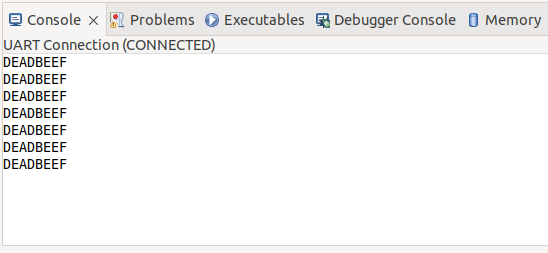
\includegraphics[width=0.7\textwidth]{anlagen/bilder/hw_test_uart}
    \caption{UART Monitorausgabe in der STMCubeIDE}
    \label{fig:impl-hw-uart-result}
\end{figure}

Die Funktionsweise des \ac{gpio}-Testprogramms ist aufgrund schlechter
Kameraverhältnisse nur schwer zu darzustellen.
Das Umschalten der LEDs ist mit bloßem Auge aber gut erkennbar.
\newline
Die Demo-Applikation des \ac{edi} Projekts konnte nicht auf dem
Entwicklungsboard ausgeführt werden.
Die \ac{hal} und \ac{cmsis} Bibliotheken konnte auf die CMake Konfiguration des
Demo Projekts übertragen werden.
Aufgrund der unerwartet hohen Komplexität und Unübersichtlichkeit der
\texttt{libopencm3} Bibliothek wird die Funktionsweise des \acl{edi} nur mit
der QEMU-Erweiterung dargestellt.


%##########################################################
% Fünftes Kapitel
%##########################################################
%!TeX root = ./../Bachelorarbeit.tex

%##########################################################
% Inhalt
%##########################################################

\clearpage
\chapter{Auswertung und Ausblick}

Die Emulation eines 32-Bit Mikrocontrollers durch das Programm QEMU bietet
viele Möglichkeiten, den aufwändigen Prozess der Embedded Software Entwicklung
zu vereinfachen.
Die Ausführung einer Embedded Software Anwendung im Kontext einer emulierten
Architekturplattform kommt einer echten Hardwareumgebung bereits sehr nahe.
Allerdings ist der Implementationsaufwand hoch.
Bereits wenig komplexe Mikrocontroller-Peripherien benötigen ein umfangreiches
Verständnis des gesamten Systems.

\section{Auswertung}

\subsection{Emulationsergebnisse}

Die Erweiterung von QEMU durch den STM32F429-\ac{soc} und die \ac{gpio}
Peripherie ermöglicht bereits jetzt eine zuverlässige Emulation des Systems.
Im Vergleich mit der QEMU-\ac{edi} Erweiterung war die Device-Erweiterung
komplexer, aber auch weniger fehleranfällig.
Sie ermöglicht die fast volle Emulation STM32F429-\ac{soc}.
Je vollständger die Implementation der Mikrocontroller-Peripherie, desto besser
kann der Test auf realer Hardware ersetzt werden.
Wie in Kapitel \ref{sec:impl-tests-emulation} gesehen werden konnte, ist eine
Ausführung einfacher Testanwendungen fast ohne Einschränkungen möglich.
Hier ist das Alter des QEMU-Projekts ein weiterer Vorteil.
Es existieren bereits viele Implementationen, die direkt für einen
Mikrocontroller genutzt werden können.
Sollte eine direkte Nutzung einer Peripherie nicht möglich sein, kann sie meist
dennoch als Vorlage für eine neue Implementation verwendet werden.
Häufig ähneln sich die Konzepte der Schnittstellen.

Das QEMU-\ac{edi} Projekt ist ebenso in der Lage, einfache Peripherie schnell
zu emulieren.
Der Ansatz der \ac{ipc}-Kommunikation ist gut dafür geeignet, kurzfristige,
schnelle Testimplementationen von Mikrocontrollern und der dazugehörigen
Peripherien zu entwickeln.
Eine unvollständige Peripherie-Abdeckung ist bei diesem Ansatz kein großes
Problem, da es einfach ist, ein neues Skript für eine neue Peripherie zu
schreiben.
Die Austauschbarkeit emulierter und hardwarebasierter Testanwendungen erhöht die
Entwicklungsgeschwindigkeit.
Die Nutzung der gleichen Schnittstellen kann beim Design von
Softwarearchitektur helfen, da die Testanwendung sowohl in der Emulation als
auch auf der echten Hardware die gleiche \enquote{logische Struktur} haben.
Es besteht ein hoher Freiheitsgrad für Implementationen.
Er wird lediglich beschränkt durch das Konzept der \ac{ipc}-Kommunikation.
Diese ist aber bereits in viele moderne Programmiersprachen gut integriert.

\subsection{Problemdiskusion}

Obwohl die Ergebnisse der QEMU-Device Erweiterung bereits eine gute Abbildung
der echten Hardware darstellen, so ist der Implementationsaufwand dennoch hoch.
Die QEMU-\acp{api} und Kommandozeilenargumente stellen mächtige Werkzeuge dar.
Allerdings können sie auch den Aufwand einer Implementation ungewollt erhöhen.
Als Beispiel hierfür sind die \textit{Properties}.
Es war nicht einfach möglich die Werte eines Objekts dynamisch zu verändern,
wie in Kapitel \ref{sec:impl-qemu-reset} dargestellt wurde.
Das schränkt den Implementationsfreiraum ein und führt zur Erhöhung der
Softwarekomplexität.
Ein weiteres Problem ist die Unvollständigkeit der Peripherie-Implementationen.
Wie in Kapitel \ref{sec:impl-tests-emulation} zu sehen, hat das Fehlen einer
wichtigen Mikrocontroller-Komponente berits große Auswirkungen auf die
Vollständigkeit der Emulation.
Je \enquote{zentraler} die Funktion der Peripherie, desto eher sollte sie
implementiert werden.
Das Alter und die Komplexität der QEMU Softwarearchitektur wirken sich
ebenfalls restriktiv auf zukünftige Implementationen aus.
Ein Beispiel hierfür ist die Nutzung der C Programmiersprache.
Es werden moderne Programmierparadigmen, wie Objektorientierte Programmierung
oder die Definition und Implementation von Schnittstellen in QEMU angewandt.
Allerdings sind diese bei weitem nicht so stark ausgeprägt wie in einer
moderneren Programmiersprache wie C++ oder Rust.
Die Fehleranfälligkeit von Programmiersprachen ohne starke Typisierung, wie
beispielsweise C, ist vergleichsweise höher als bei Sprachen mit starker
Typisierung\cite{GithubProgrammingLanguagesStudy}.
Eine weitere Hürde bei der QEMU-Device Erweiterung ist die Bereitstellung von
\enquote{Simluationsdaten}.
Es ist in QEMU nicht ohne weiteres möglich, Testdaten für eine Peripherie
bereitzustellen.
Für einfache Schnittstellen wie \ac{uart} ist dies noch kein großes Problem.
Je komplexer die Peripherie wird, desto höher sind die Anforderungen an eine
vollständige Emulation.
Es bedingt beispielsweise die Implementation komplexer
\textit{Device-Backends}, welche den Gesamtaufwand der Emulation deutlich
erhöhen.

Auch die Nutzung moderner Programmierparadigmen ist keine Garantie für eine
Verringerung der Komplexität.
Ein Beispiel hierfür ist die im \ac{edi} Demo-Projekt eingeführte
Abstraktionsebene für die Austauschbarkeit der darunter liegenden
Implementation.
Diese wird ermöglicht durch die Definition von Schnittstellen und damit der Austauschbarkeit einer Implementation.
% und damit austauschbarkeit der Implemntation
Es erhöht aber auch die Komplexität der Gesamtanwendung.
Sie verfehlt darüber hinaus das verfehlt aber das Ziel der
vollständigen Abstraktion der echten Hardware durch eine emulierte Umgebung.
Das Ziel einer Emulation sollte es sein, Software ohne jegliche Anpassung
ausführen zu können, egal ob in einer emulierten Umgebung oder auf echter
Hardware.
Die Abstraktion der darunter liegenden Implementation ermöglicht zwar schnelles
\enquote{Prototyping}, allerdings wird die Software dadurch schwerer
verständlich.
Die Komplexität von \ac{ipc}-Kommunikation kann ebenfalls eine Einstiegshürde
sein.
Sowhol die Warbarkeit, als auch Erweiterbarkeit von Software wird dadurch im
schlimmsten Fall ebenfalls vermindert.
Wichtig ist hierbei eine klare Definition der verwendeten Schnittstellen und die
Nutzung ausgereifter, möglichst fehlerfreier Software.
Im Falle der QEMU-\ac{edi} Erweiterung wird dies komplizierter, da das Projekt
auf den Stand der Version 4.2.0 festgesetzt ist.
Das Projekt muss ohne Bugfixes und neue Features auskommen.
Ein Update auf eine neuere Version wäre sehr aufwändig.

\section{Ausblick}

Die Implementation einer \ac{gpio} Peripherie ist nur ein erster Schritt für
die vollständige Emulation eines Mikrocontroller.
\newline
Im nächsten Schritt sollte zuerst zentrale, wichtige Peripherie implementiert
werden.
Ein Beispiel hierfür ist \ac{rcc} oder des Interrupt Watchdog, beziehungsweise
Window Watchdog.
Darüber hinaus sollten die bestehenden Peripherien vervollständigt werden.
Ein Beispiel hierfür die \enquote{alternative Funktion} der
\ac{gpio}-Peripherie.
Sind diese Peripherie Geräte implementiert, sollten die  Ethernet und \ac{can}
Schnittstellen folgen.
Beide sind von zentraler Beudetung im Kontext moderener Embedded Software.
\newline
Abseits davon wäre die Bereitstellung von Testdaten eine wichtige Erweiterung.
Eine grafische Darstellung eines Entwicklungsboards in Verbindung mit der
Emulation durch QEMU könnte helfen, das Zusammenspiel zwischen Mikrocontroller
udes nd Peripherie besser zu veranschaulichen.
Darüber hinaus ist die einfache Integration in automatische Testgenerierung,
beziehungsweise Integrationtesting ein breites Feld, was von den breiten
Möglichkeiten der Emulation stark profitieren würde.


%##########################################################
% Literatur
%##########################################################
%!TeX root = ./../Bachelorarbeit.tex

%##########################################################
% Inhalt
%##########################################################
\printbibliography[title={Literaturverzeichnis}, heading=bibintoc]


%##########################################################
% Anhang - nicht verwendete Anhangsseiten bitte kommentieren
%##########################################################
\appendix
\pagenumbering{Roman}
\setcounter{page}{1}

%!TeX root = ./../Bachelorarbeit.tex

%##########################################################
% Inhalt
%##########################################################
\clearpage
\chapter{Anhang -\ Abbildungen}

%!TeX root = ./../Bachelorarbeit.tex

%##########################################################
% Inhalt
%##########################################################
\clearpage
\chapter{Anhang -\ Tabellen}

%!TeX root = ./../Bachelorarbeit.tex

%##########################################################
% Inhalt
%##########################################################
\clearpage
\chapter{Anhang -\ Quelltexte}

\begin{minipage}{\linewidth}
\lstinputlisting[language=c,numbers=none,
                label={lst:qemu-gpio-memops},
                linerange={384-399,419-427},
                caption=Konfiguration der \ac{mmio}-Speicherregion des GPIO-Devices]
                {anlagen/qemu-device/stm32f429_gpio.c}
\end{minipage}

\begin{minipage}{\linewidth}
\lstinputlisting[language=c,numbers=none,
                label={lst:qemu-gpio-vmstates},
                linerange={364-382},
                caption=Definition der \texttt{VMStates} zum Laden/Speichern der Zustände eines Objekts]
                {anlagen/qemu-device/stm32f429_gpio.c}
\end{minipage}

\lstinputlisting[caption=STM32F429 SoC Header Datei,
                language=c,
                label={lst:qemu-soc-header}]
                {anlagen/qemu-device/stm32f429_soc.h}

\lstinputlisting[caption=STM32F429 GPIO Device Header Datei,
                language=c,
                label={lst:qemu-gpio-header}]
                {anlagen/qemu-device/stm32f429_gpio.h}

\lstinputlisting[caption=Skript zur Ausführung von QEMU mit Firmware,
                language=sh,
                label={lst:qemu-test-script}]
                {anlagen/qemu-device/stm32f429_gpio.h}


% ***********************************************
\end{document}
% ***********************************************
